\documentclass[12pt,letterpaper]{article}

\usepackage[margin=0.77in]{geometry}
\usepackage{amsmath,amssymb}
\usepackage{graphicx}
\usepackage{subcaption}
\usepackage{enumitem}
\usepackage{xcolor}
\usepackage{booktabs}
\usepackage{listings}
\usepackage[numbers,sort]{natbib}
\usepackage{hyperref}
\usepackage{tcolorbox}
\hypersetup{pdfborderstyle={/S/U/W 1}}
\title{464 A2}
\author{Nahum }
\date{November 2026}

\setlength{\parindent}{0pt}
\setlength{\parskip}{4pt}
% Long code and file names cannot be hyphenated; let TeX loosen a line instead of running past the margin.
\setlength{\emergencystretch}{3em}
\clubpenalty=10000
\widowpenalty=10000
\displaywidowpenalty=10000
\setlist[itemize]{label=$\square$, itemsep=10pt, parsep=4pt, topsep=6pt}

\colorlet{codekeyword}{blue!70!black}
\colorlet{codecomment}{green!40!black}
\colorlet{codestring}{red!60!black}

\lstdefinestyle{code}{
    basicstyle=\small\ttfamily,
    backgroundcolor=\color{black!5},
    frame=single,
    framerule=0pt,
    framesep=6pt,
    xleftmargin=6pt,
    xrightmargin=6pt,
    aboveskip=12pt,
    belowskip=12pt,
    keywordstyle=\color{codekeyword},
    commentstyle=\color{codecomment},
    stringstyle=\color{codestring},
    columns=fullflexible,
    keepspaces=true,
    showstringspaces=false
}
\lstdefinestyle{bash}{style=code, language=bash, morekeywords={bash}}
\lstdefinestyle{python}{style=code, language=Python}

% Answer area for students. The argument is the minimum height;
% the box grows with its content.

% A shape id written vertically, as a row label of the results overview.
\newcommand{\shapeid}[1]{\rotatebox[origin=c]{90}{\texttt{#1}}}


\begin{document}


\section*{Results Overview}

% Fill in the scores from each metrics.json, and the mean of each column.
\begin{table}[h]
      \centering
      \footnotesize
      \setlength{\tabcolsep}{5pt}
      \caption{Surface and edge Chamfer distance of every method on the six evaluation shapes, in grid units.}
      \label{tab:overview}
      \begin{tabular}{lcccccccccc}
            \toprule
                              & \multicolumn{2}{c}{Exact DC} & \multicolumn{2}{c}{Approx.\ DC} & \multicolumn{2}{c}{NDC}                                          \\
            \cmidrule(lr){2-3} \cmidrule(lr){4-5} \cmidrule(lr){6-7} 
            Shape             & Surface                      & Edge                            & Surface                 & Edge                    & Surface                        & Edge  \\
            \midrule
            \texttt{00003173} &0.00231973&0.05153349&0.01022575&0.4941155&0.0536468&0.587450027\\
            \texttt{00004857} &0.0013773775&0.05181375&0.01525701&0.267304&0.055745&0.4116344451\\
            \texttt{00006462} &0.00396455&0.0675192&0.01244857&0.205705&0.0709120&0.661999881\\
            \texttt{00007496} &0.002528900&0.0323729&0.0089086&0.257420&0.0447992&0.633496403\\
            \texttt{00008714} &0.002497305& 0.049456&0.01615323&0.278172&0.0673449&0.499617278\\
            \texttt{00009943} &0.00432913&0.042536221& 0.0128382&0.275712&0.05765277&0.801475882\\
            \midrule
            Mean              &0.00283615&0.0293631451&0.01093426&0.29640475&0.058350111&0.599278986016&         &      &         &      \\
            \bottomrule
      \end{tabular}
\end{table}

% Replace each \screenshot with \includegraphics[width=0.168\linewidth]{<your screenshot>}.
\begin{figure}[h]
      \centering
      \footnotesize
      \setlength{\tabcolsep}{10pt}
      \begin{tabular}{c@{\hspace{4pt}}ccc}
                               & Exact DC    & Approx.\ DC & NDC\\
            \shapeid{00003173} & 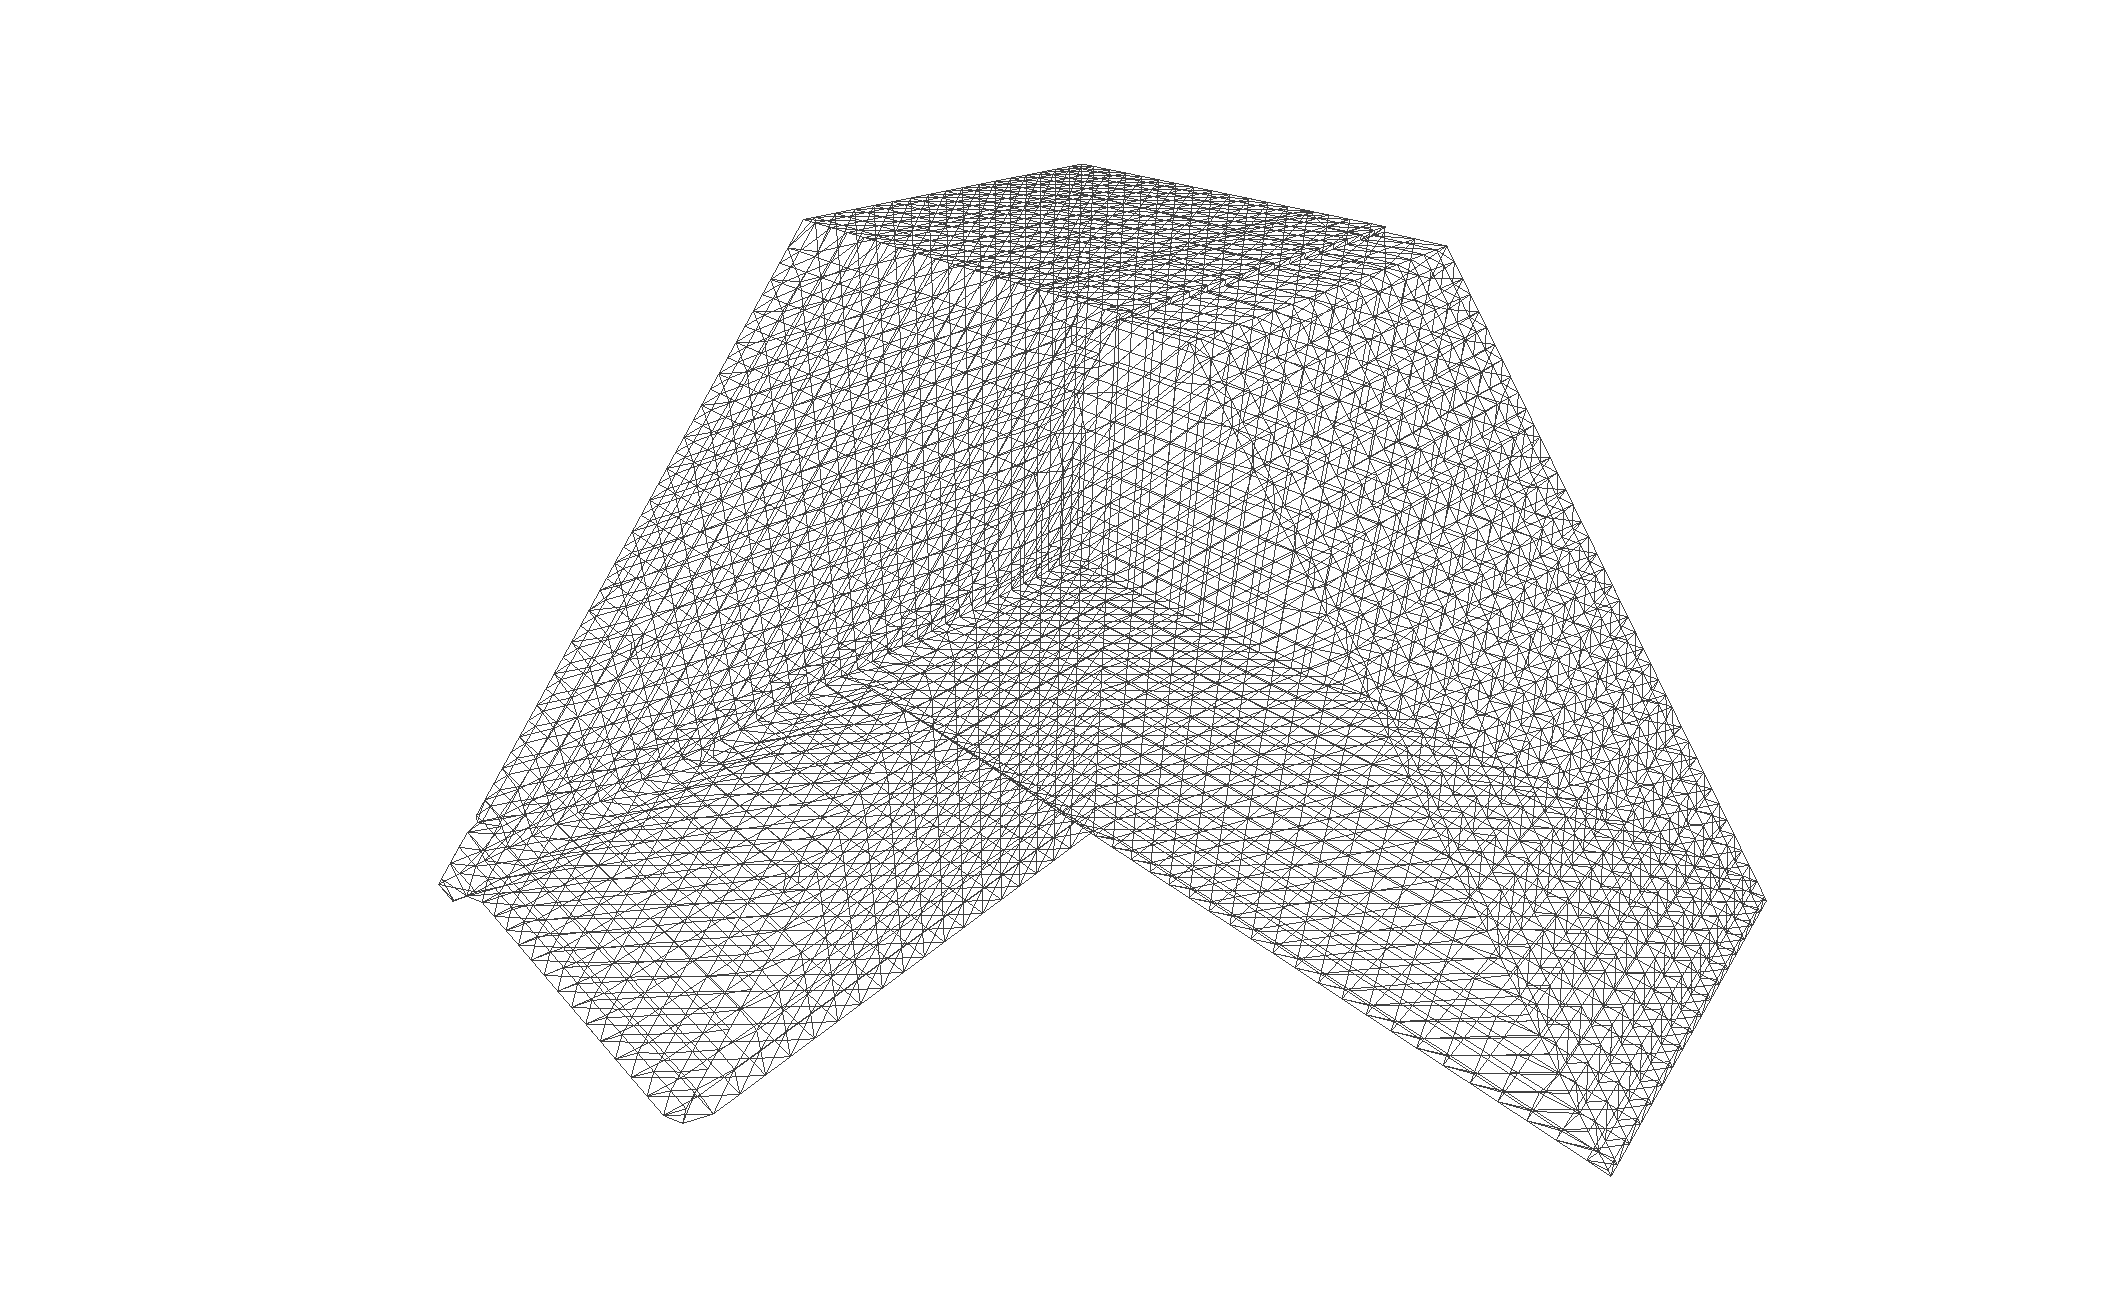
\includegraphics[width=0.25\linewidth]{3173_exact_p113.png} & 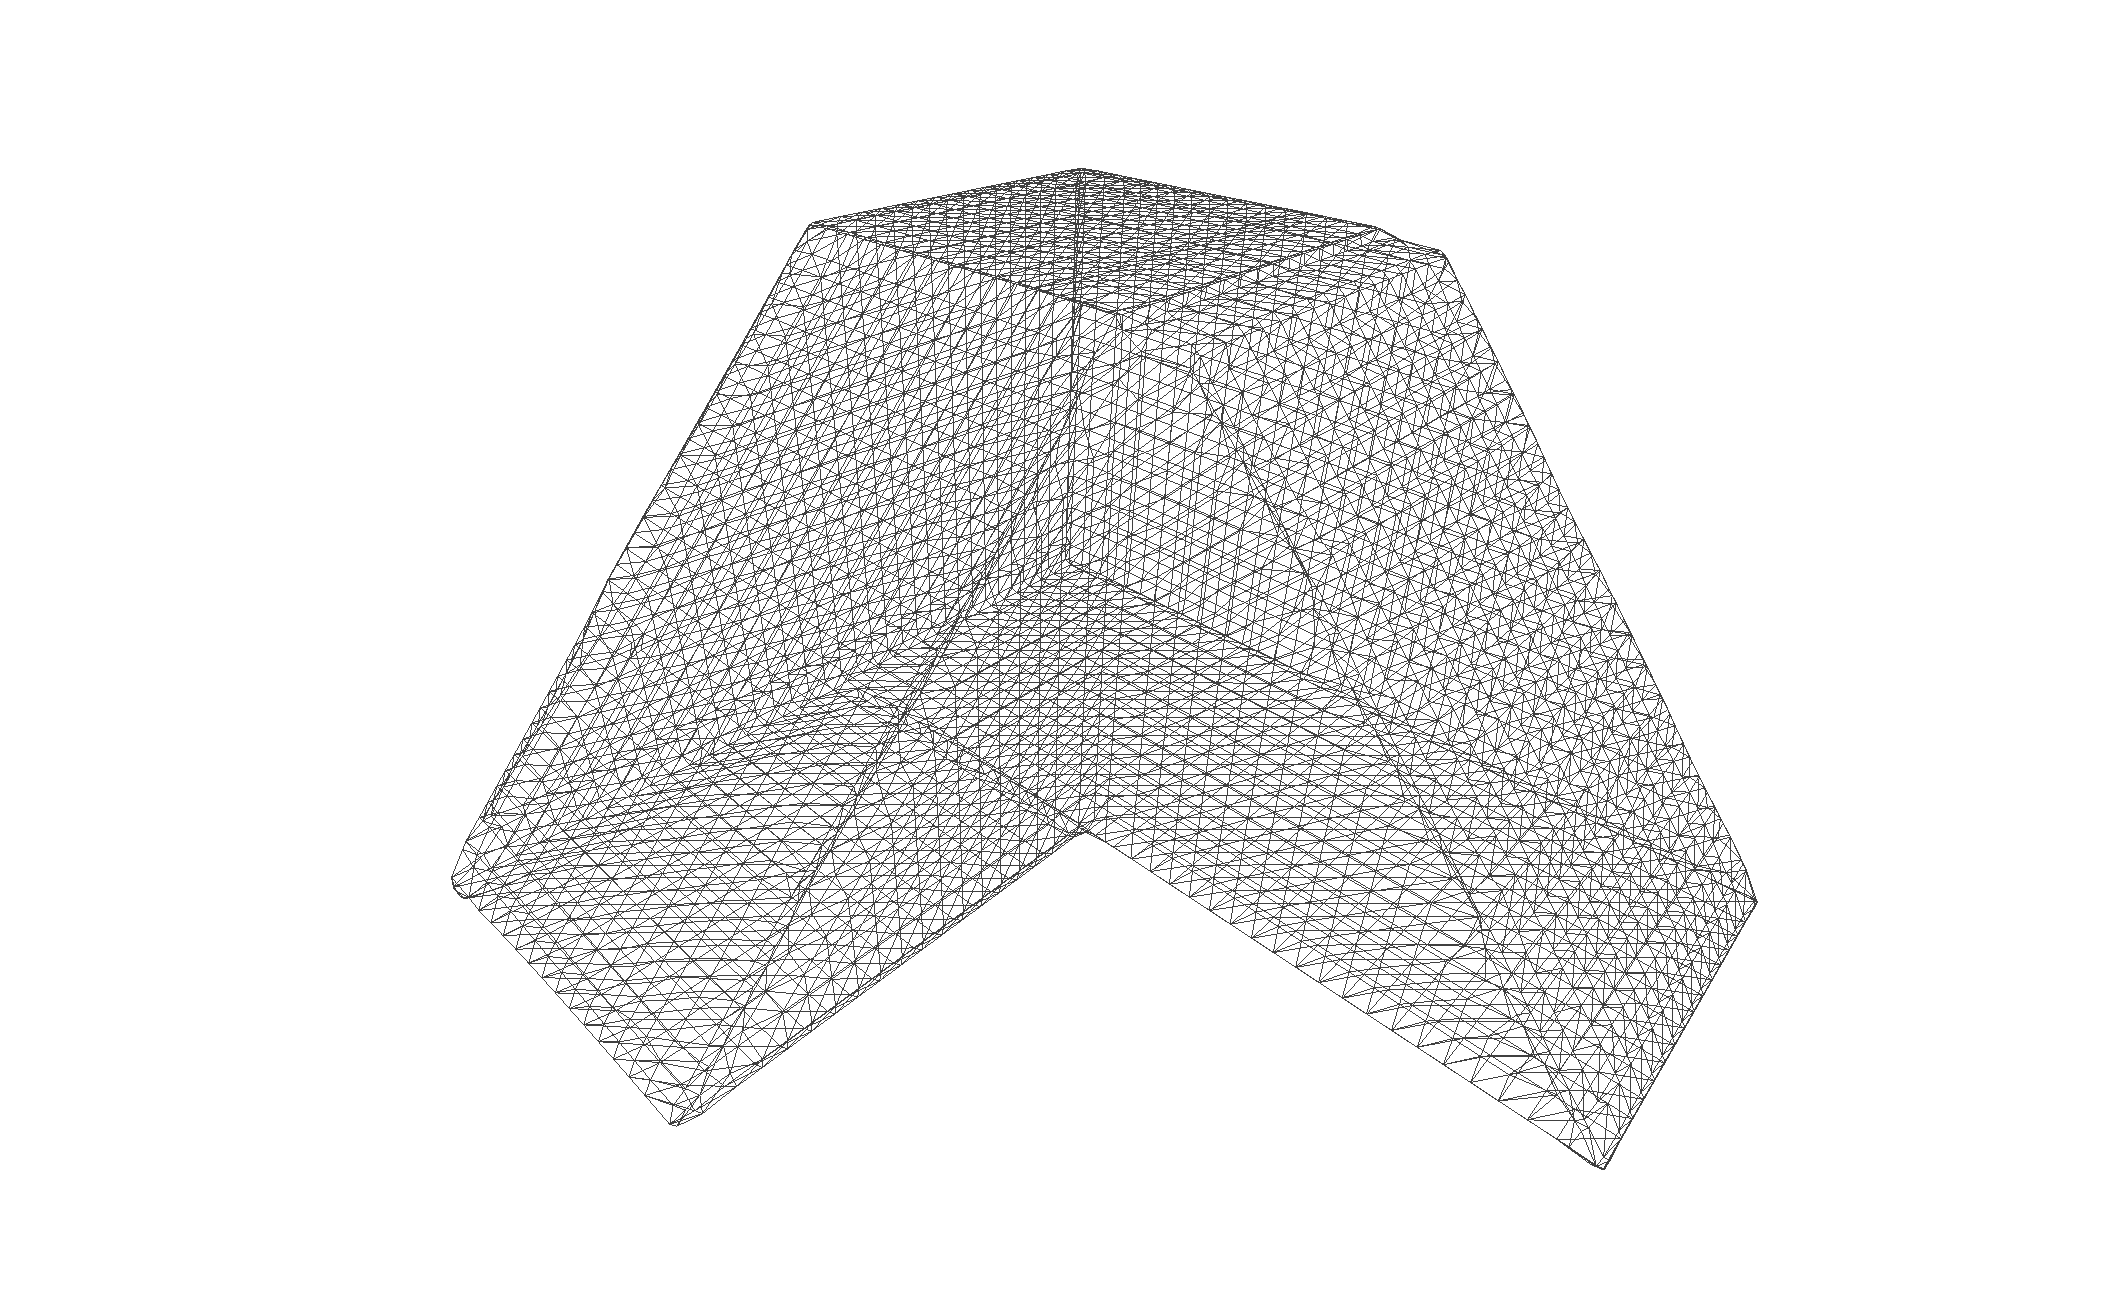
\includegraphics[width=0.25\linewidth]{3173_estimate_p114.png} & 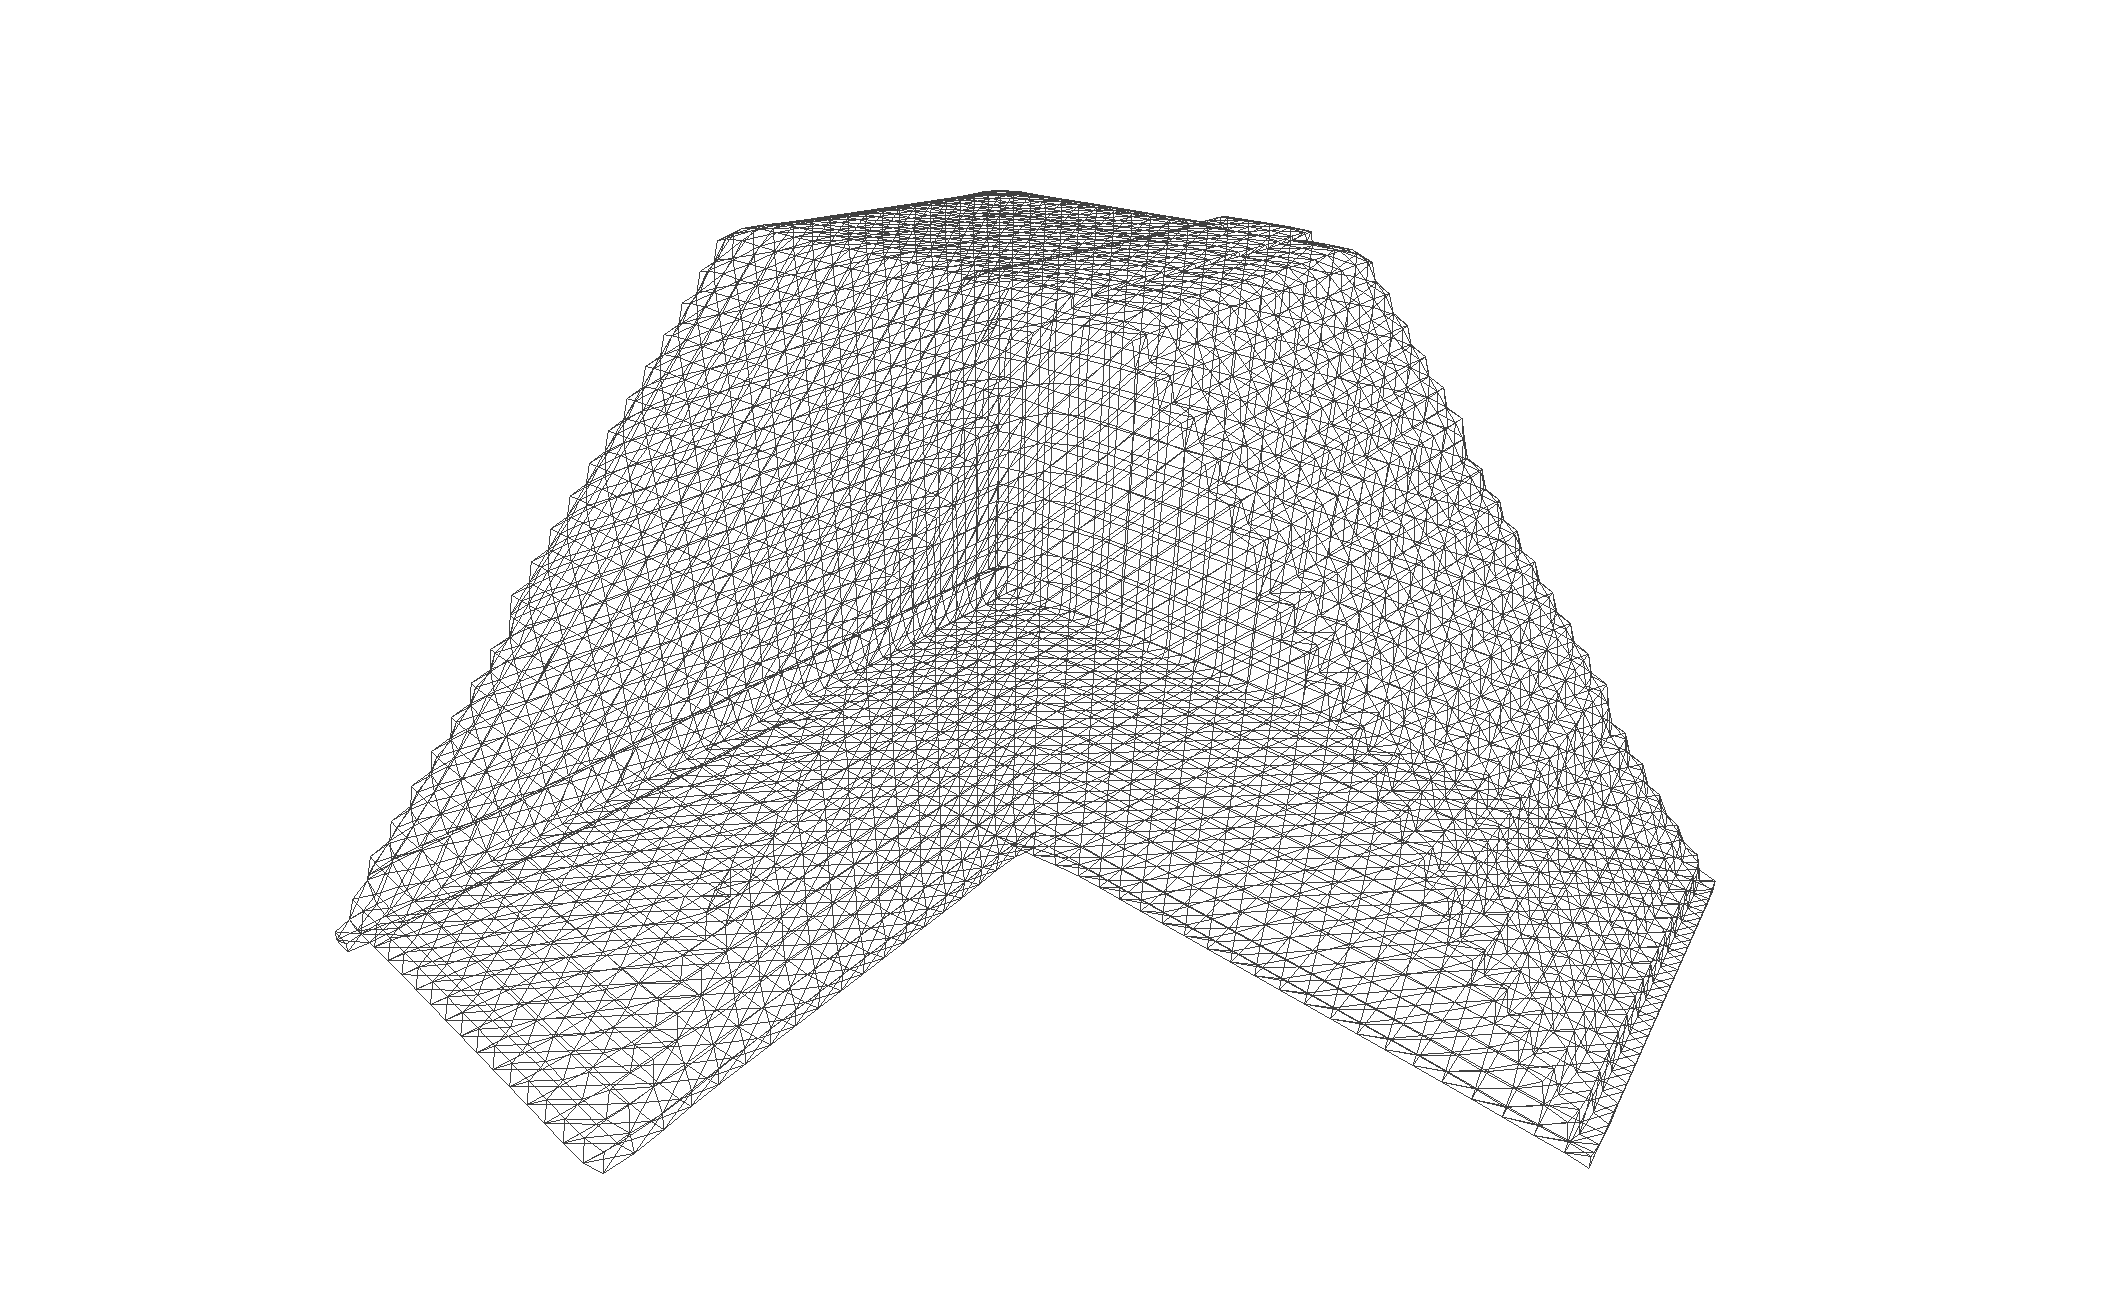
\includegraphics[width=0.25\linewidth]{3173_neural02.png}\\
            \shapeid{00004857} & 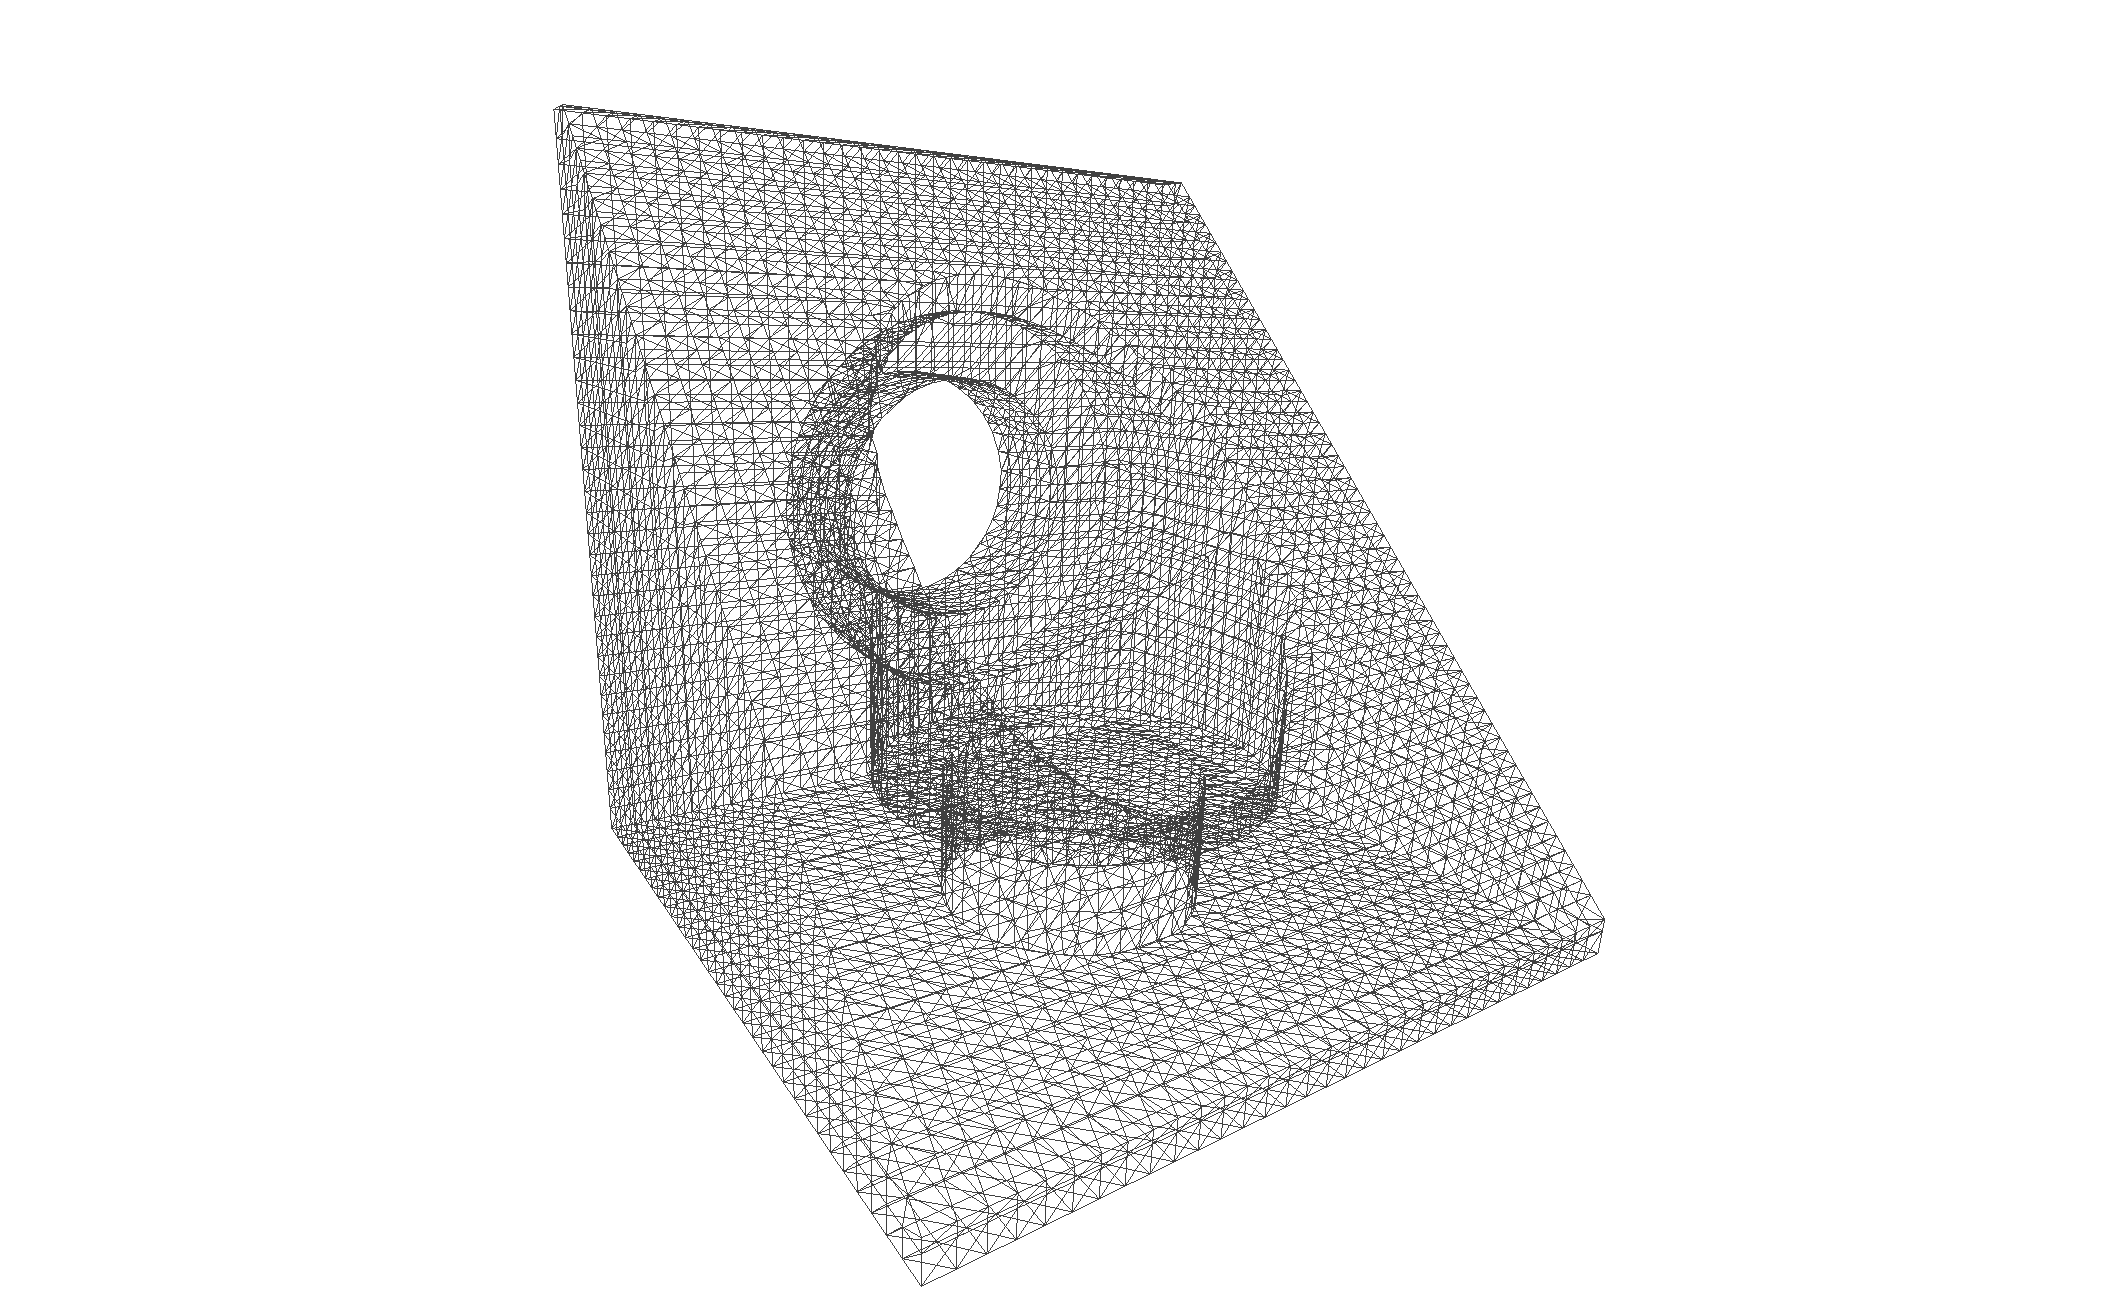
\includegraphics[width=0.25\linewidth]{4857_exact_p111.png} & 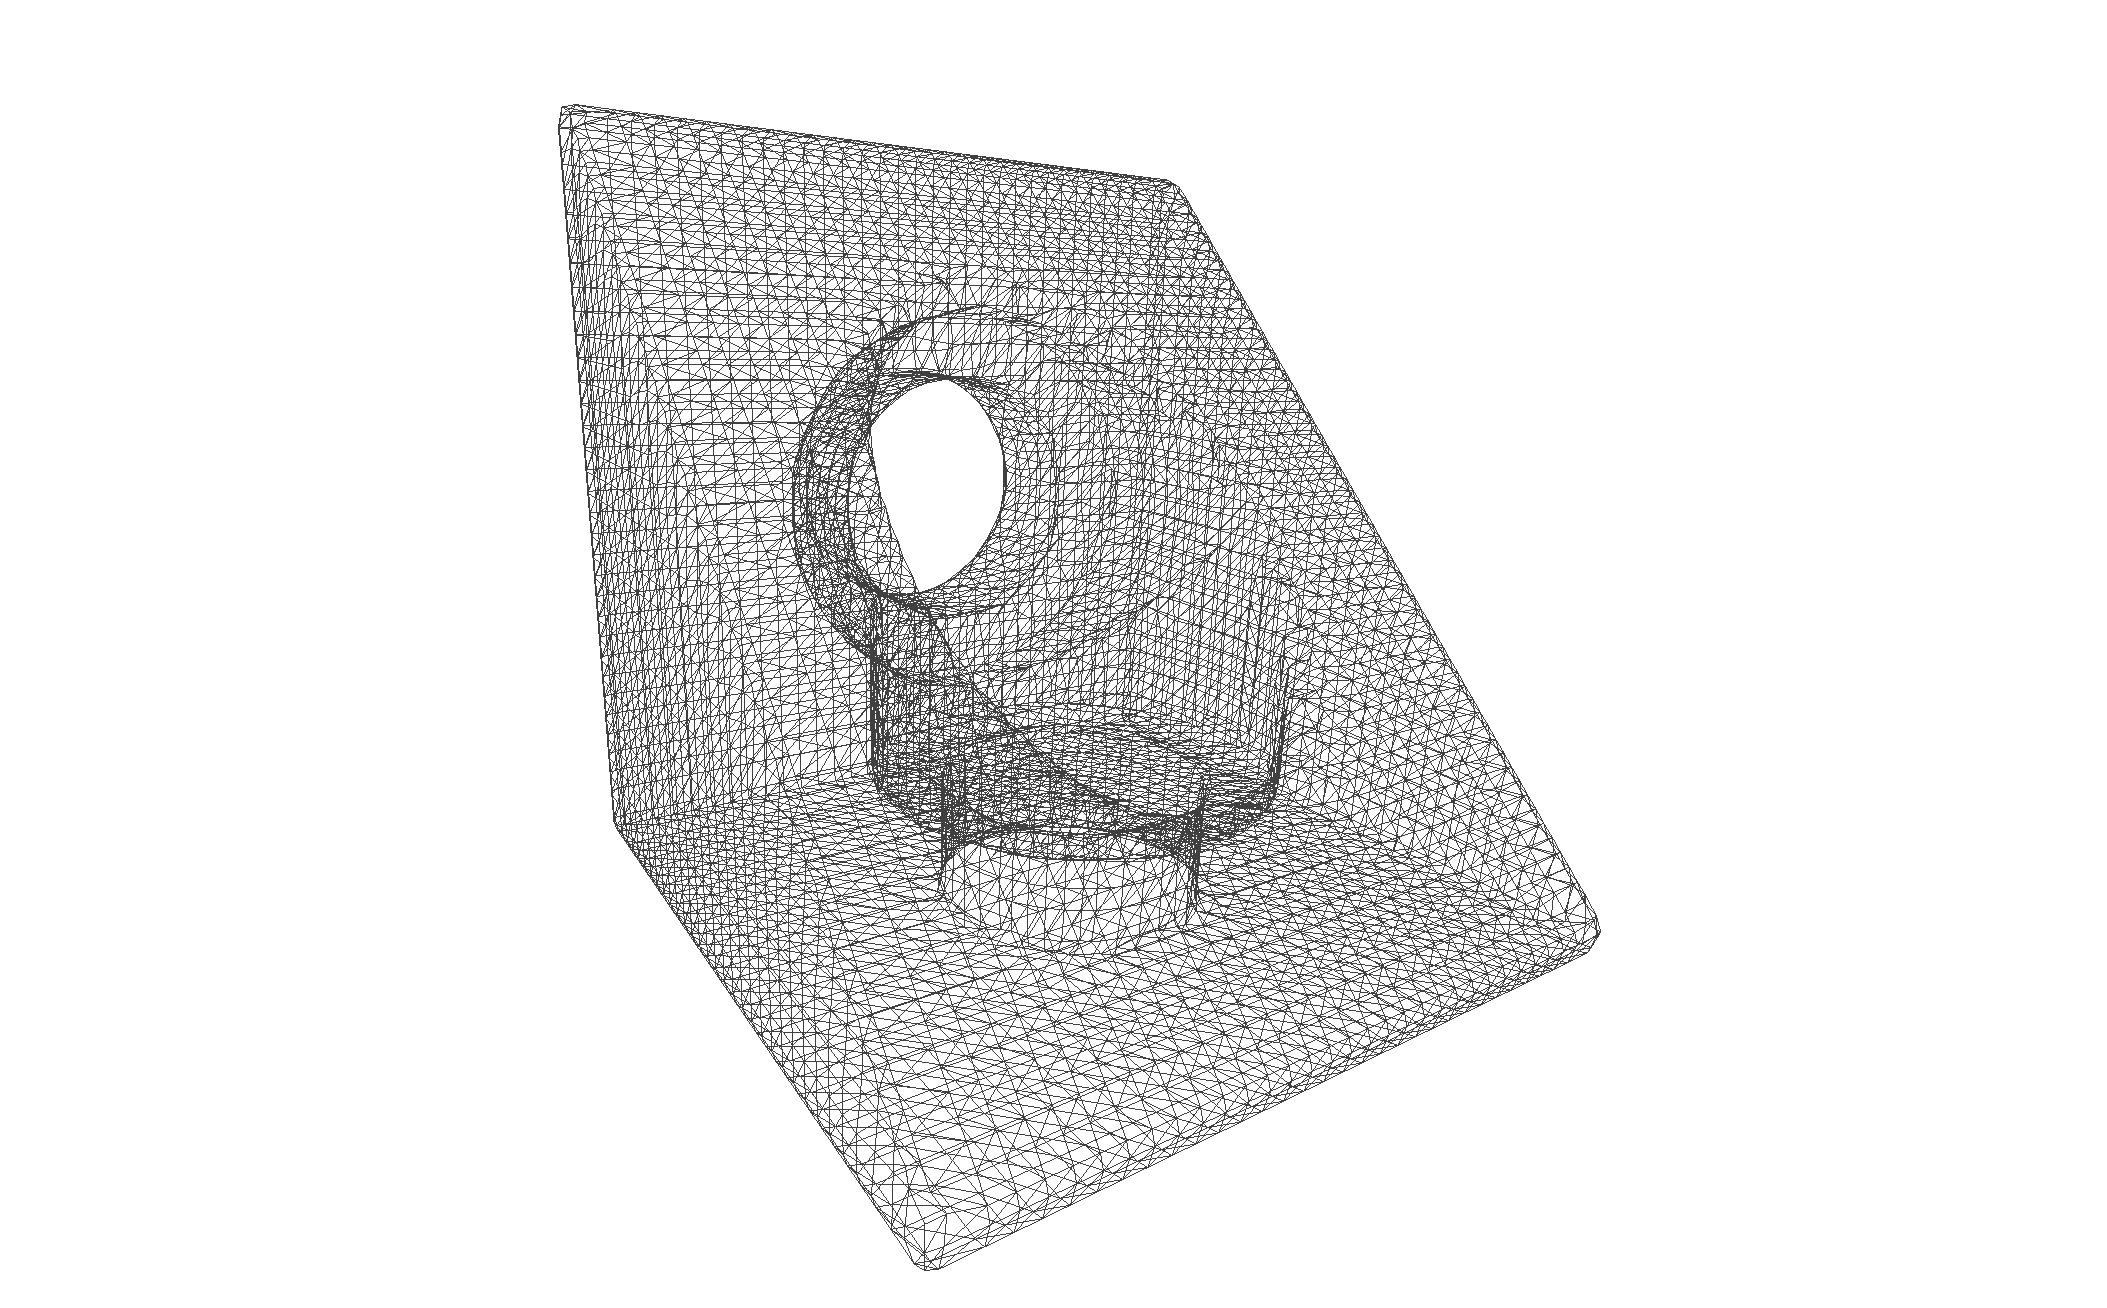
\includegraphics[width=0.25\linewidth]{4857_estimate_p112.png} & 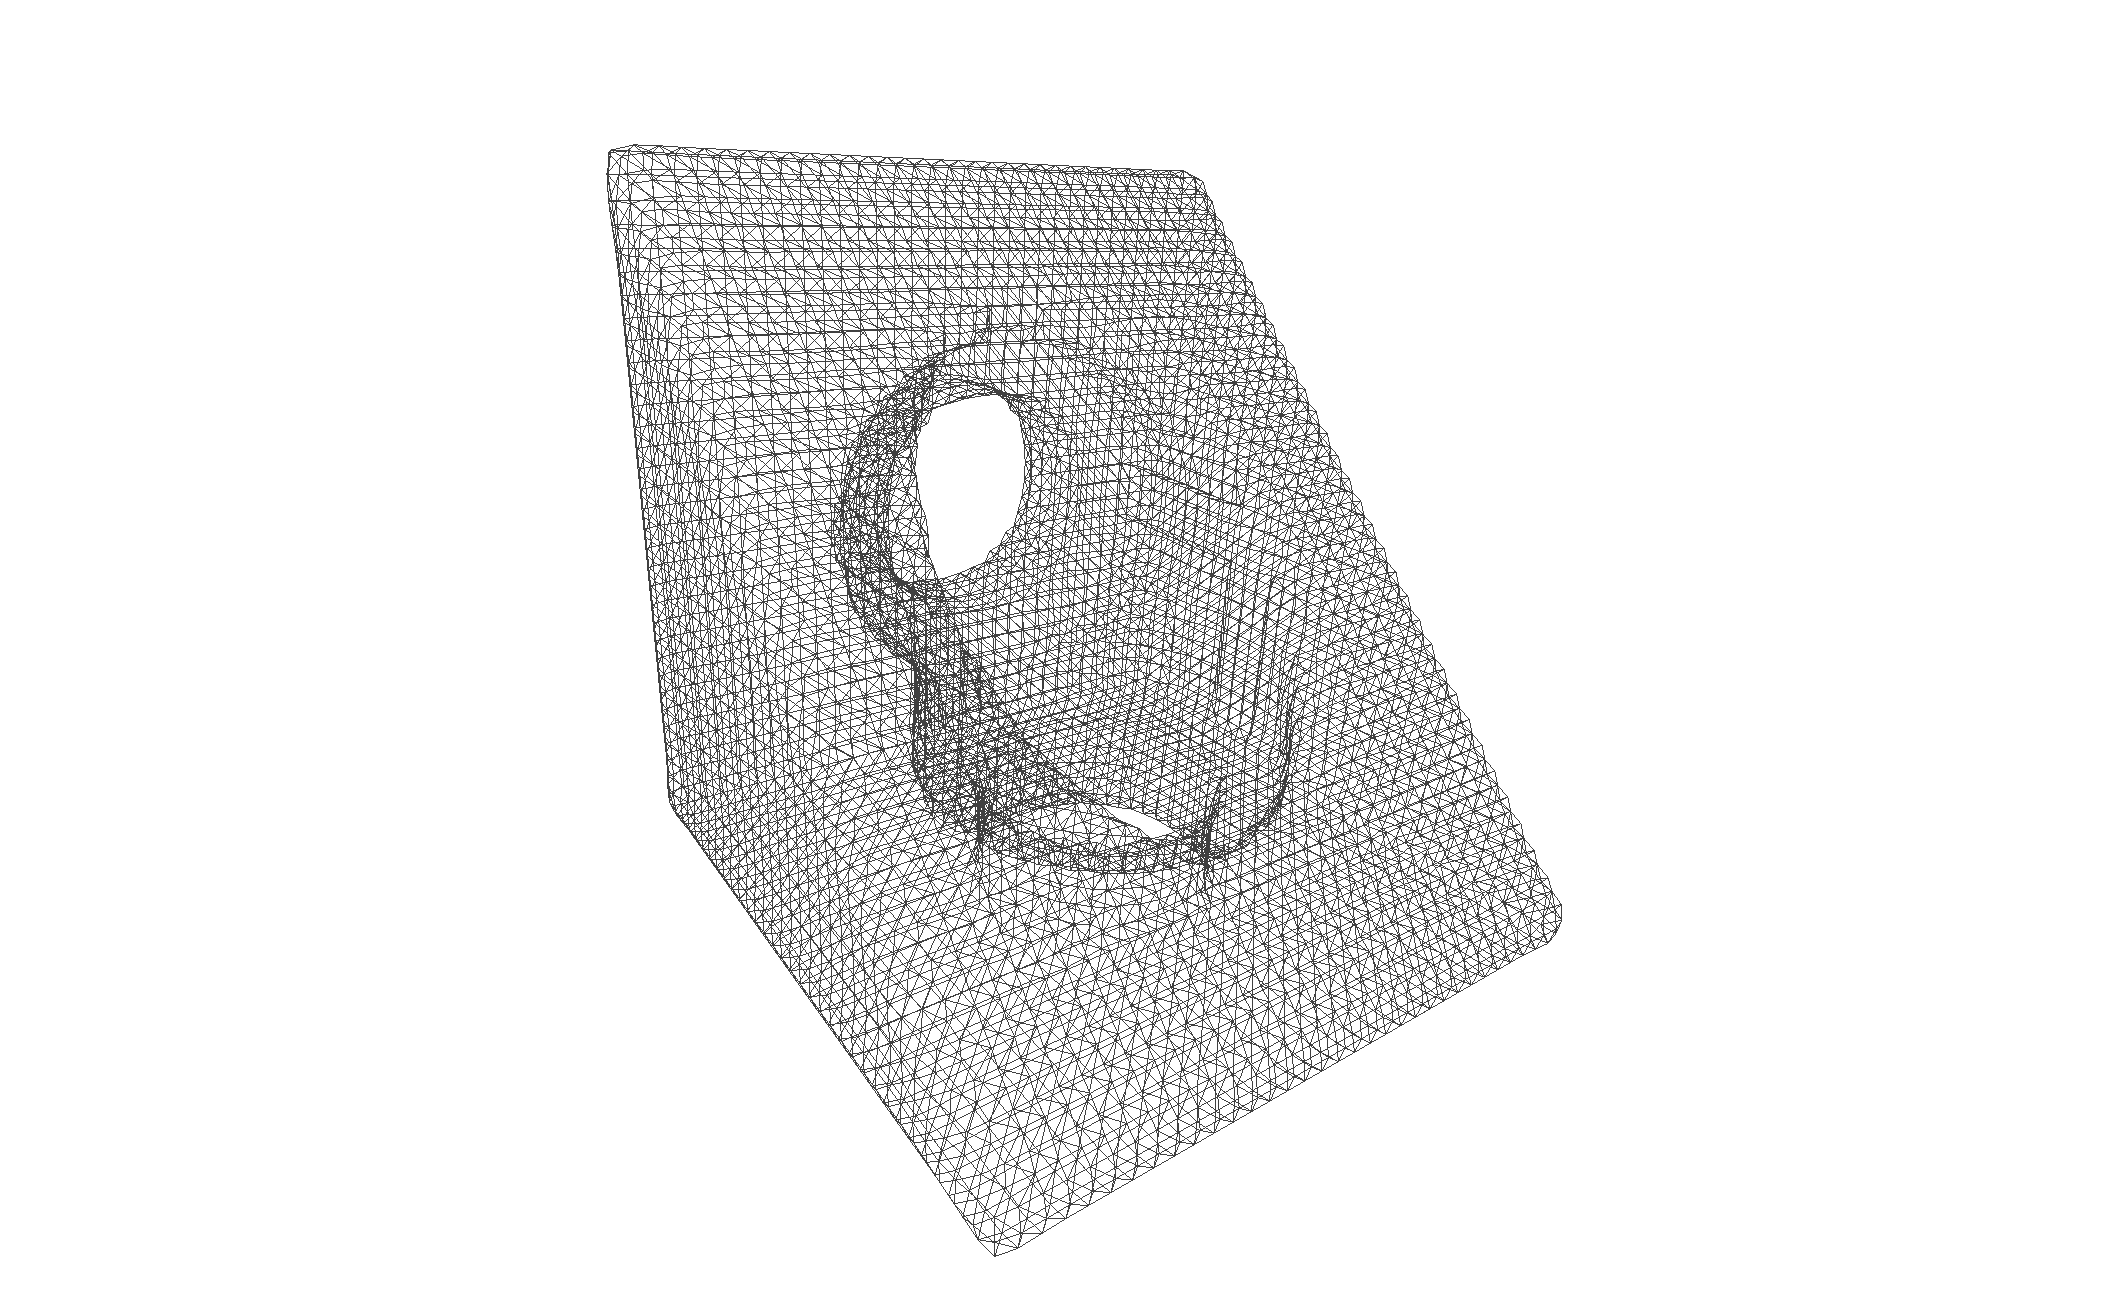
\includegraphics[width=0.25\linewidth]{4857_neural03.png}\\
            \shapeid{00006462} & 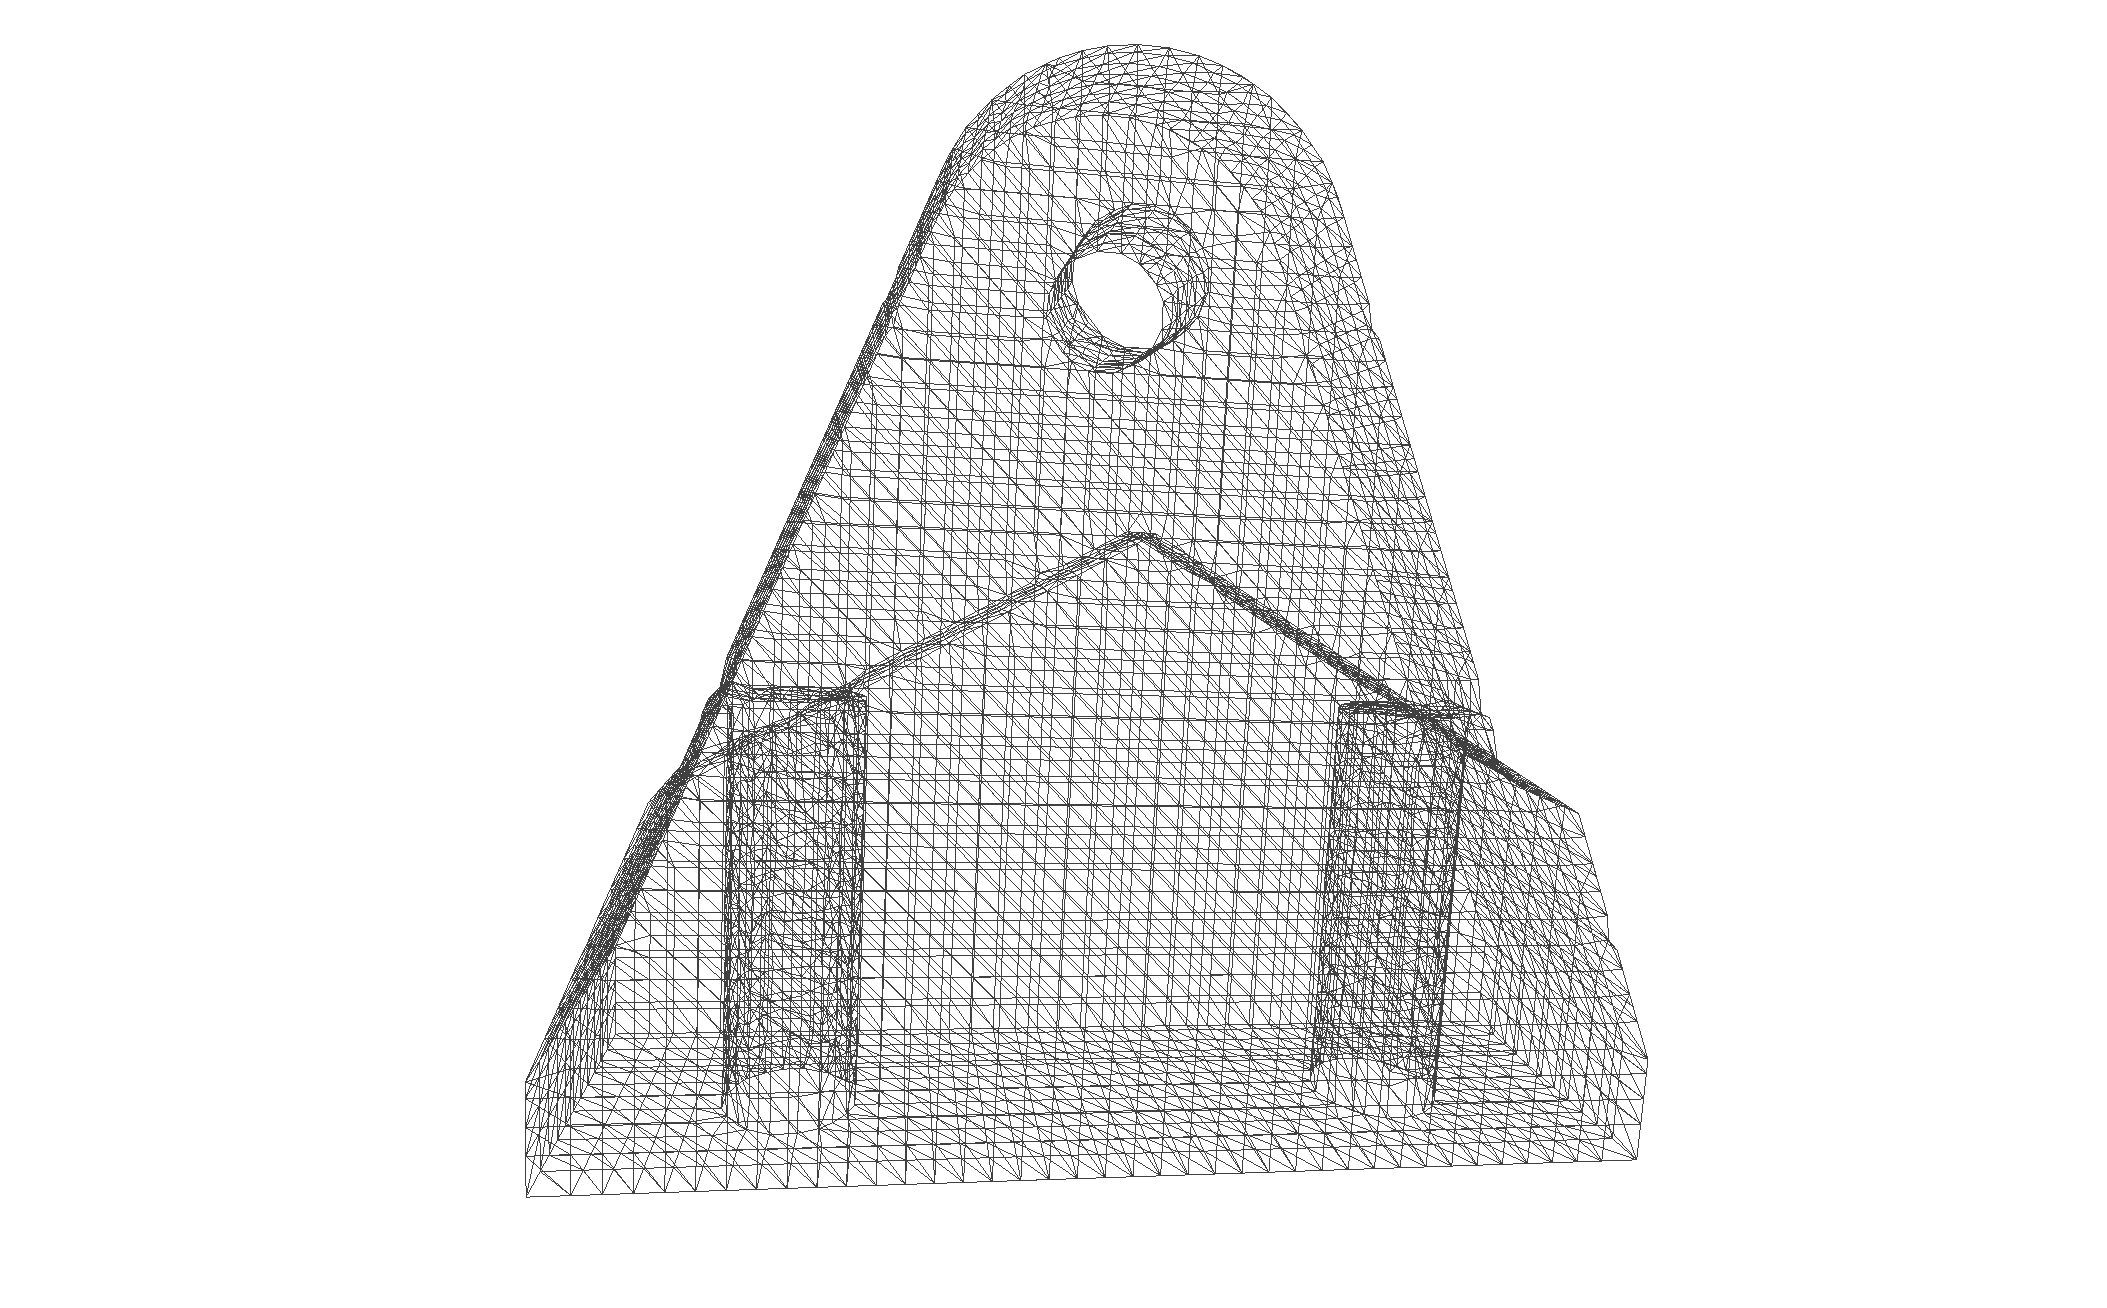
\includegraphics[width=0.25\linewidth]{64642_exact_p109.png} & 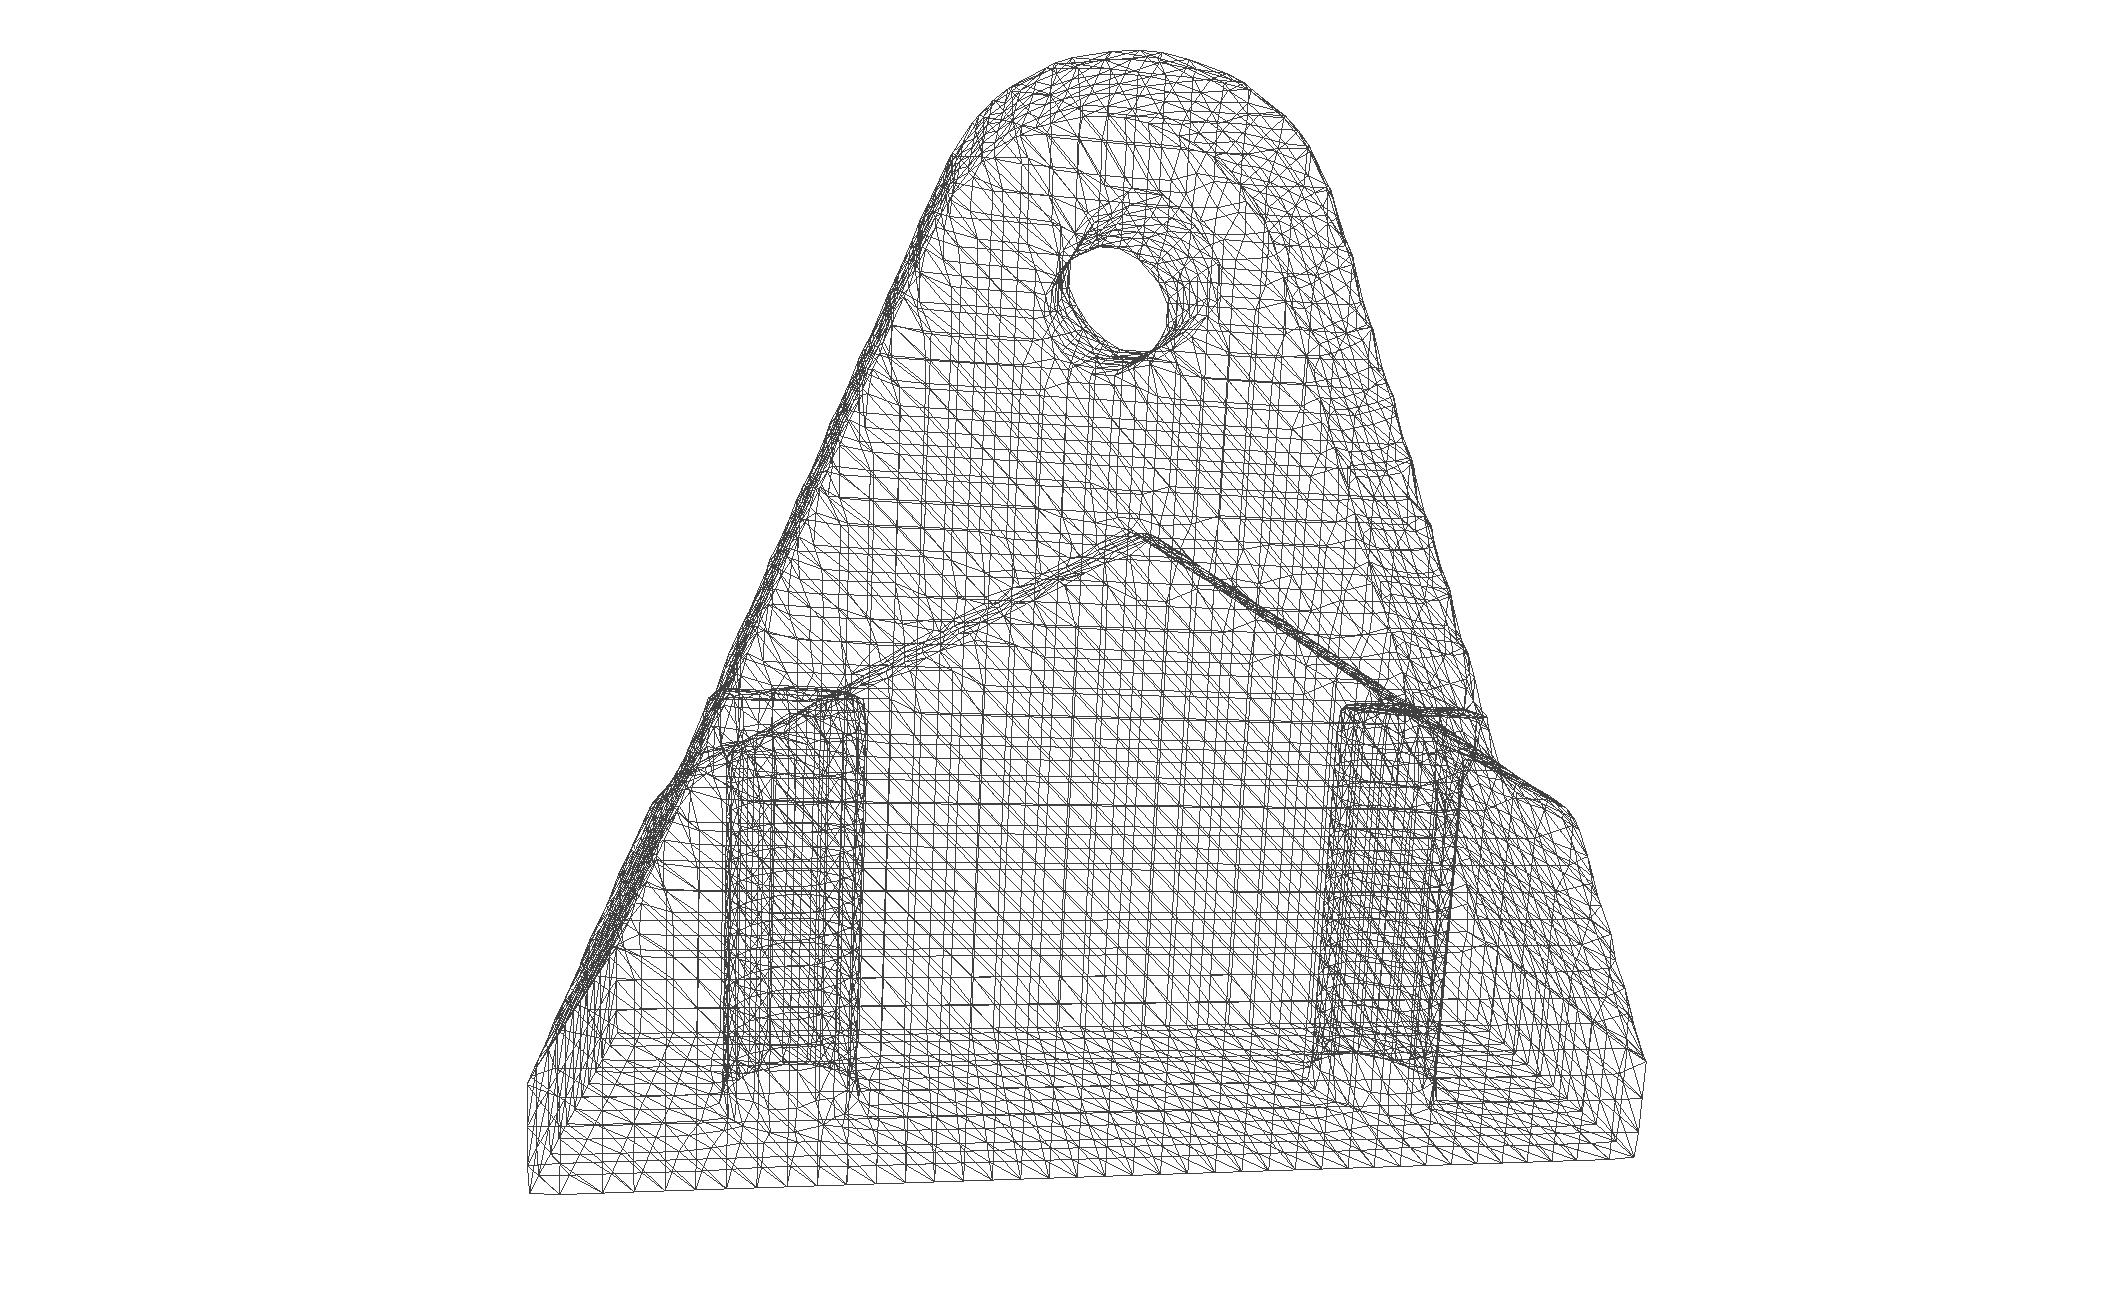
\includegraphics[width=0.25\linewidth]{64642_estimate_p110.png} & 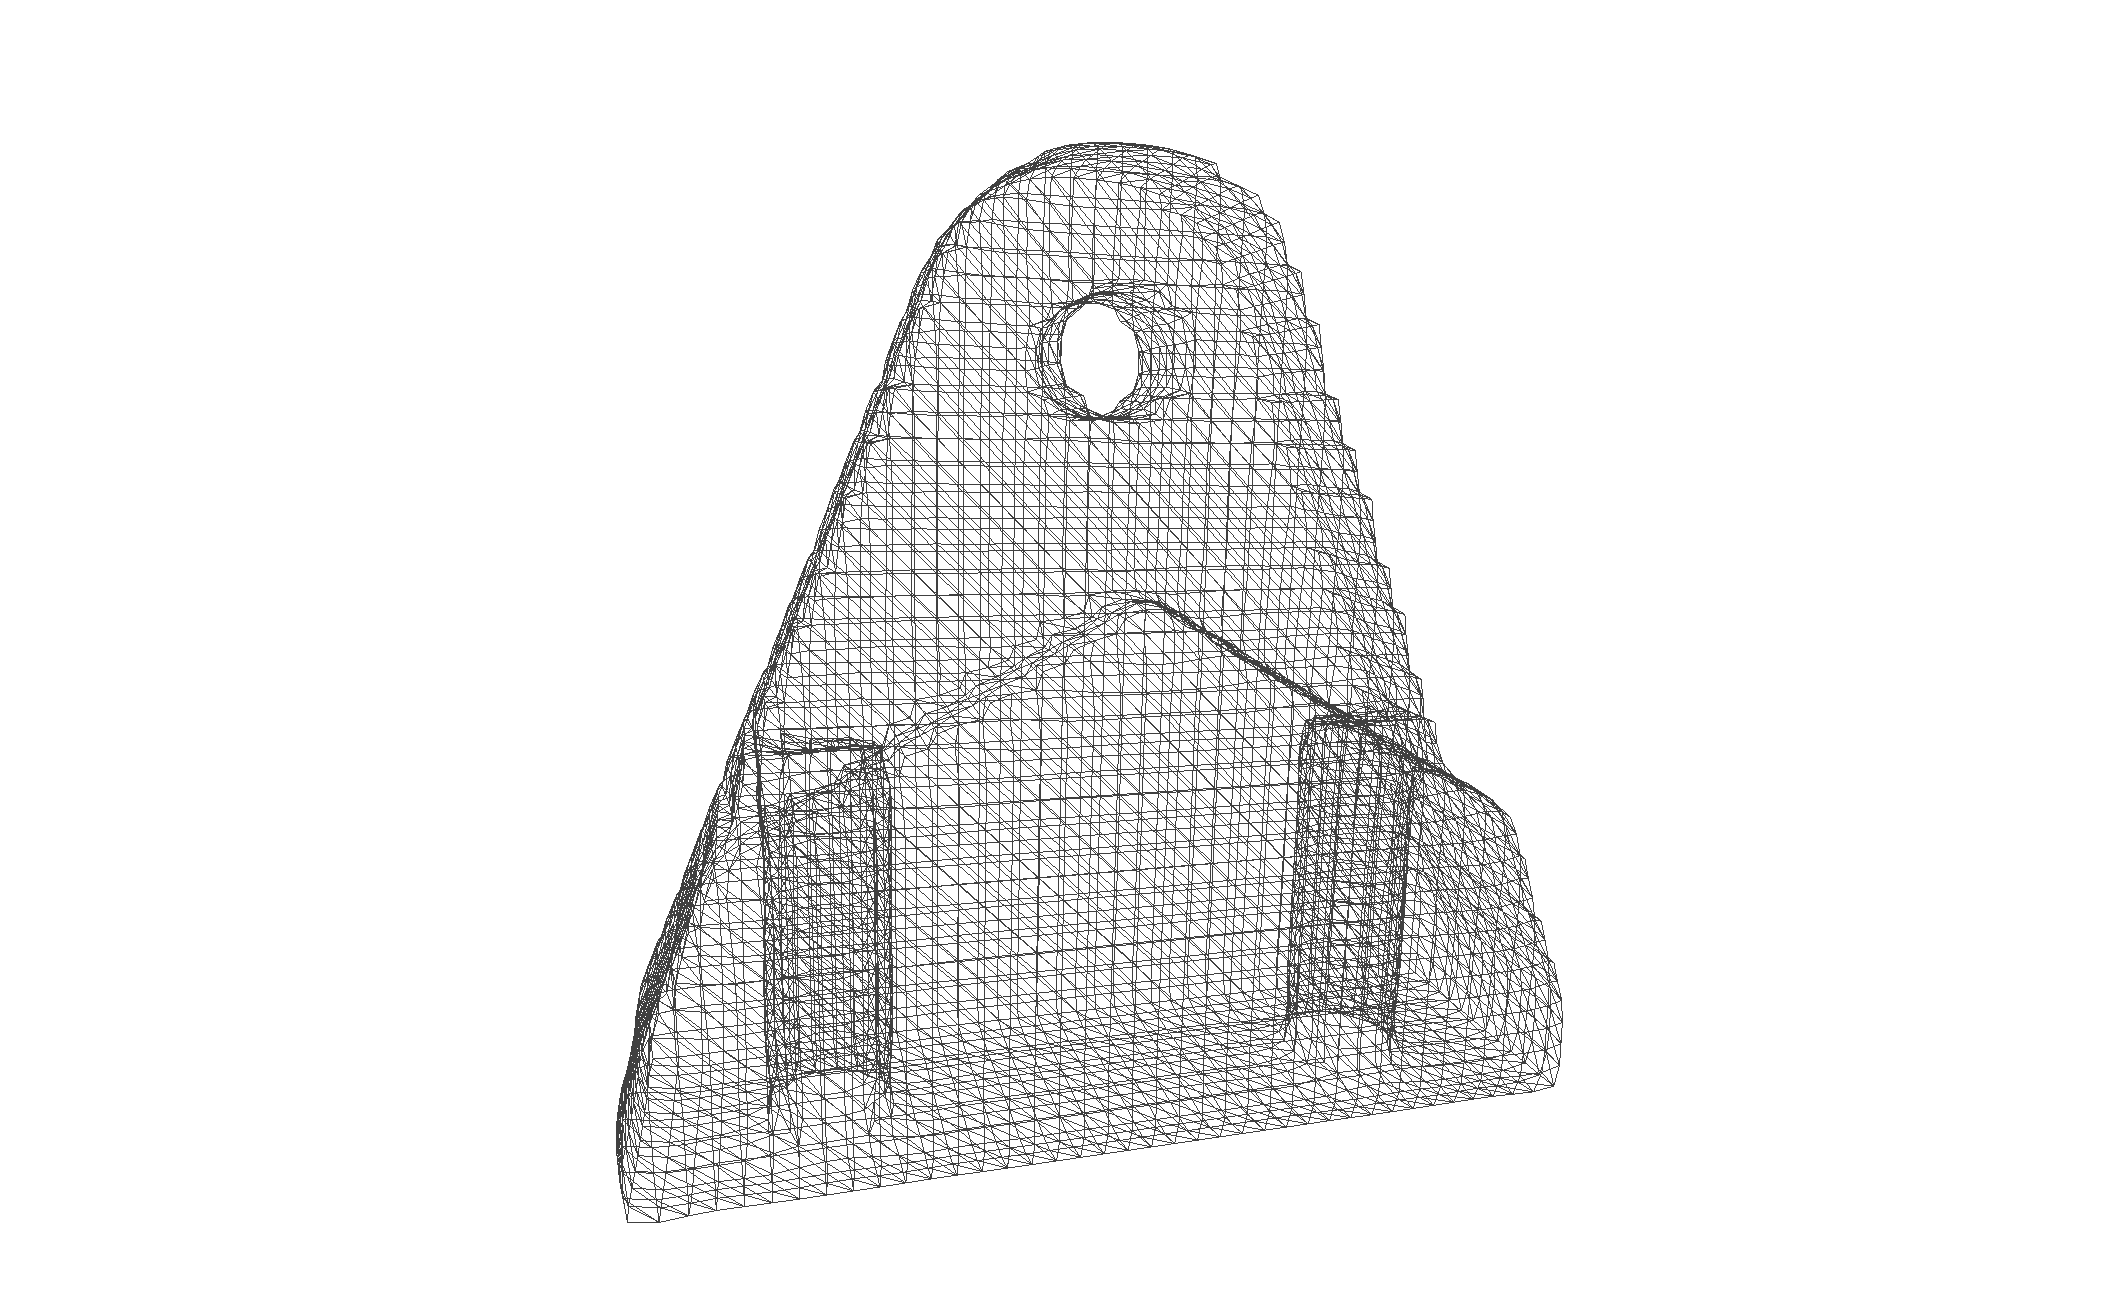
\includegraphics[width=0.25\linewidth]{6462_neural04.png}\\
            \shapeid{00007496} & 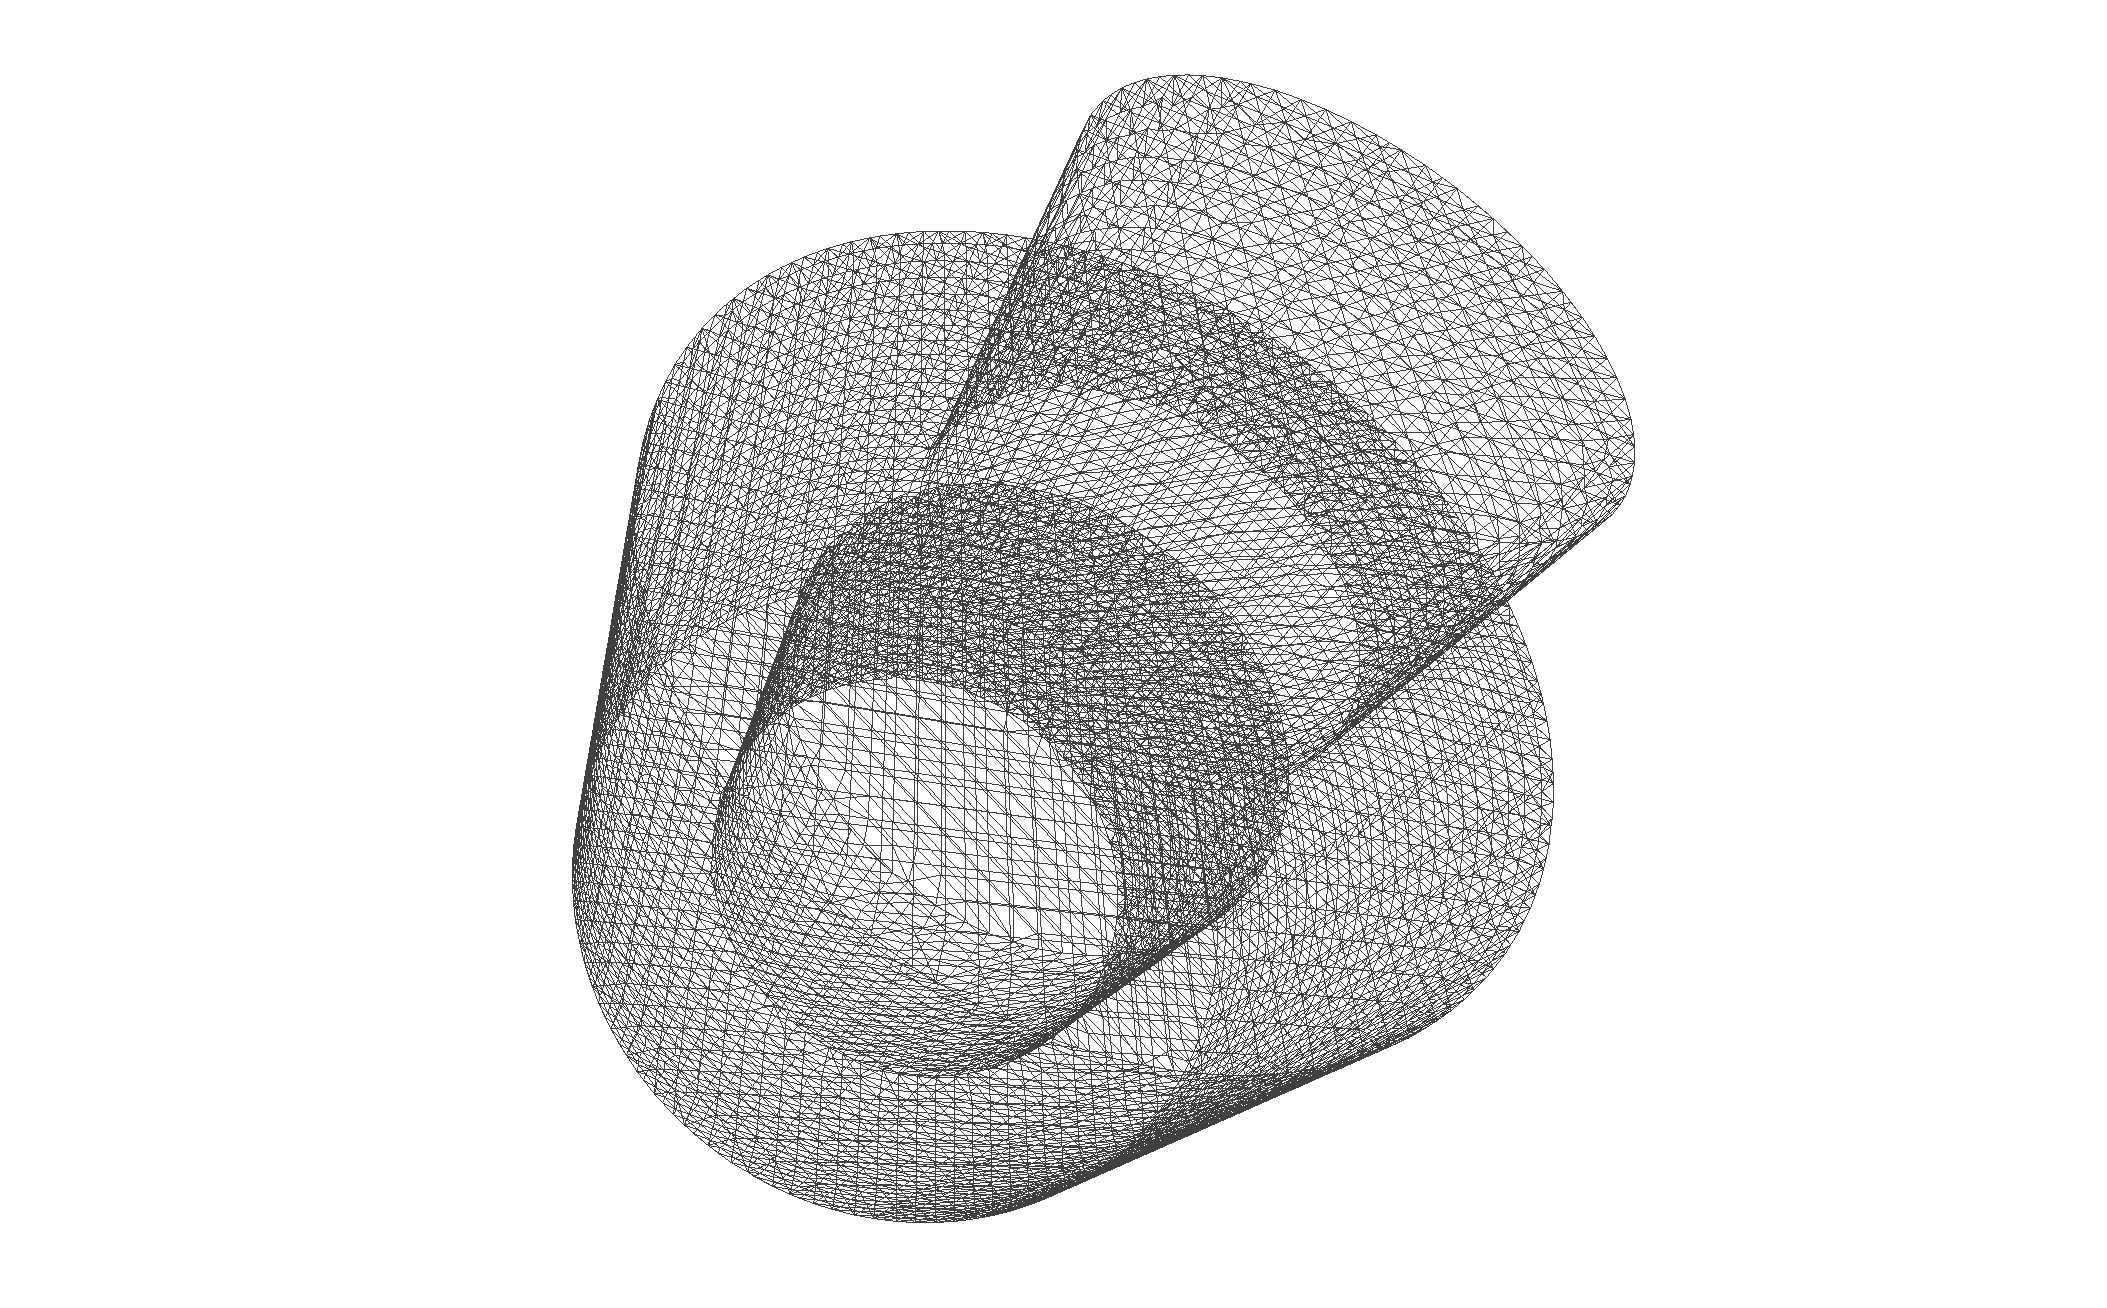
\includegraphics[width=0.25\linewidth]{7496_exact_p107.png} & 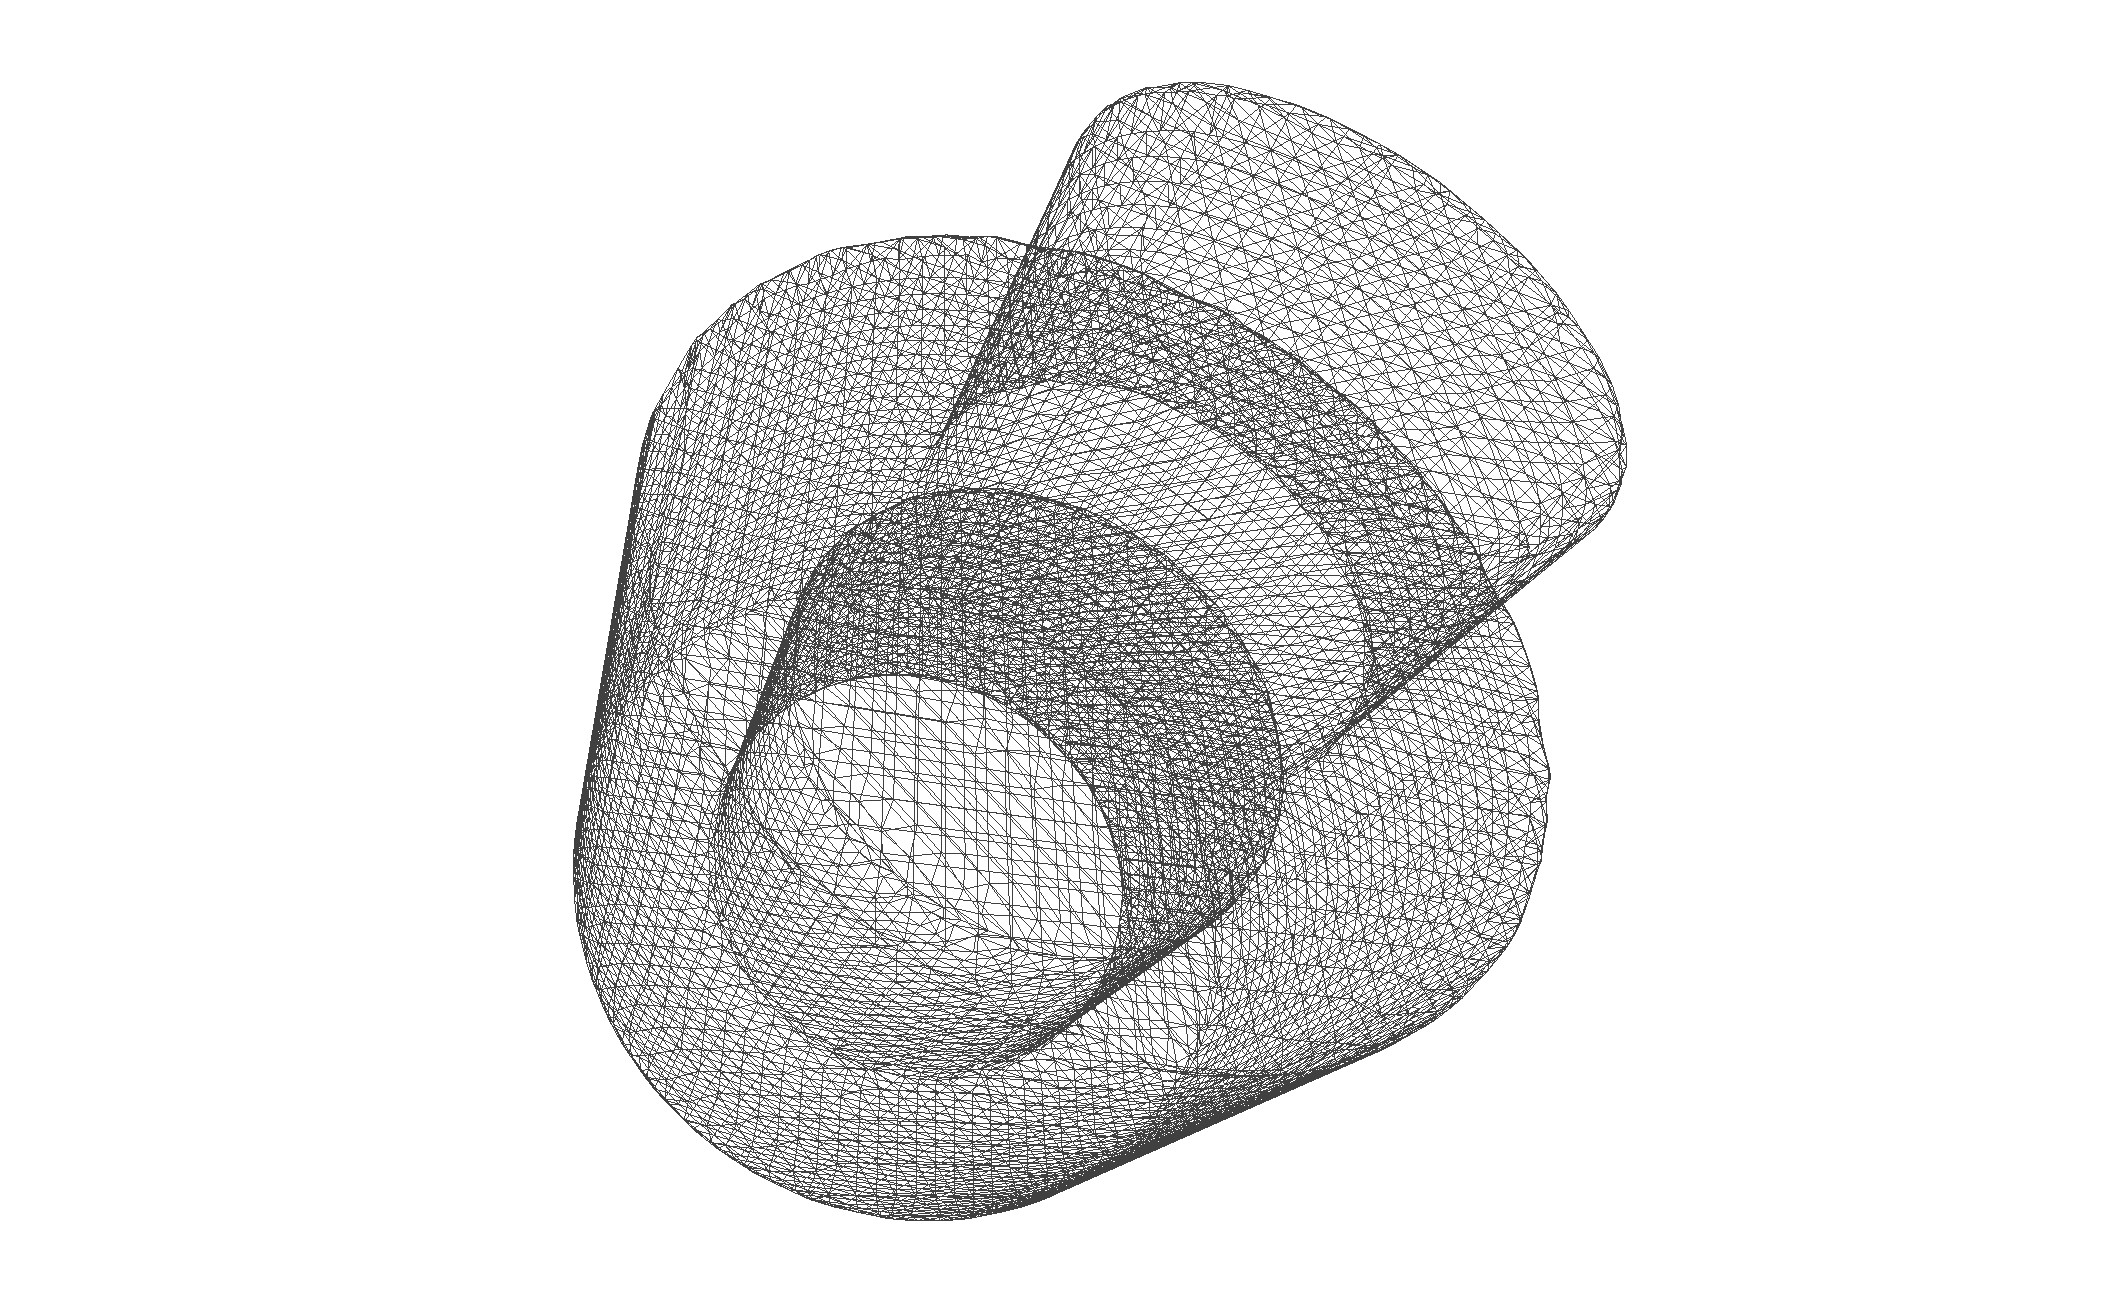
\includegraphics[width=0.25\linewidth]{7496_estimate_p108.png} & 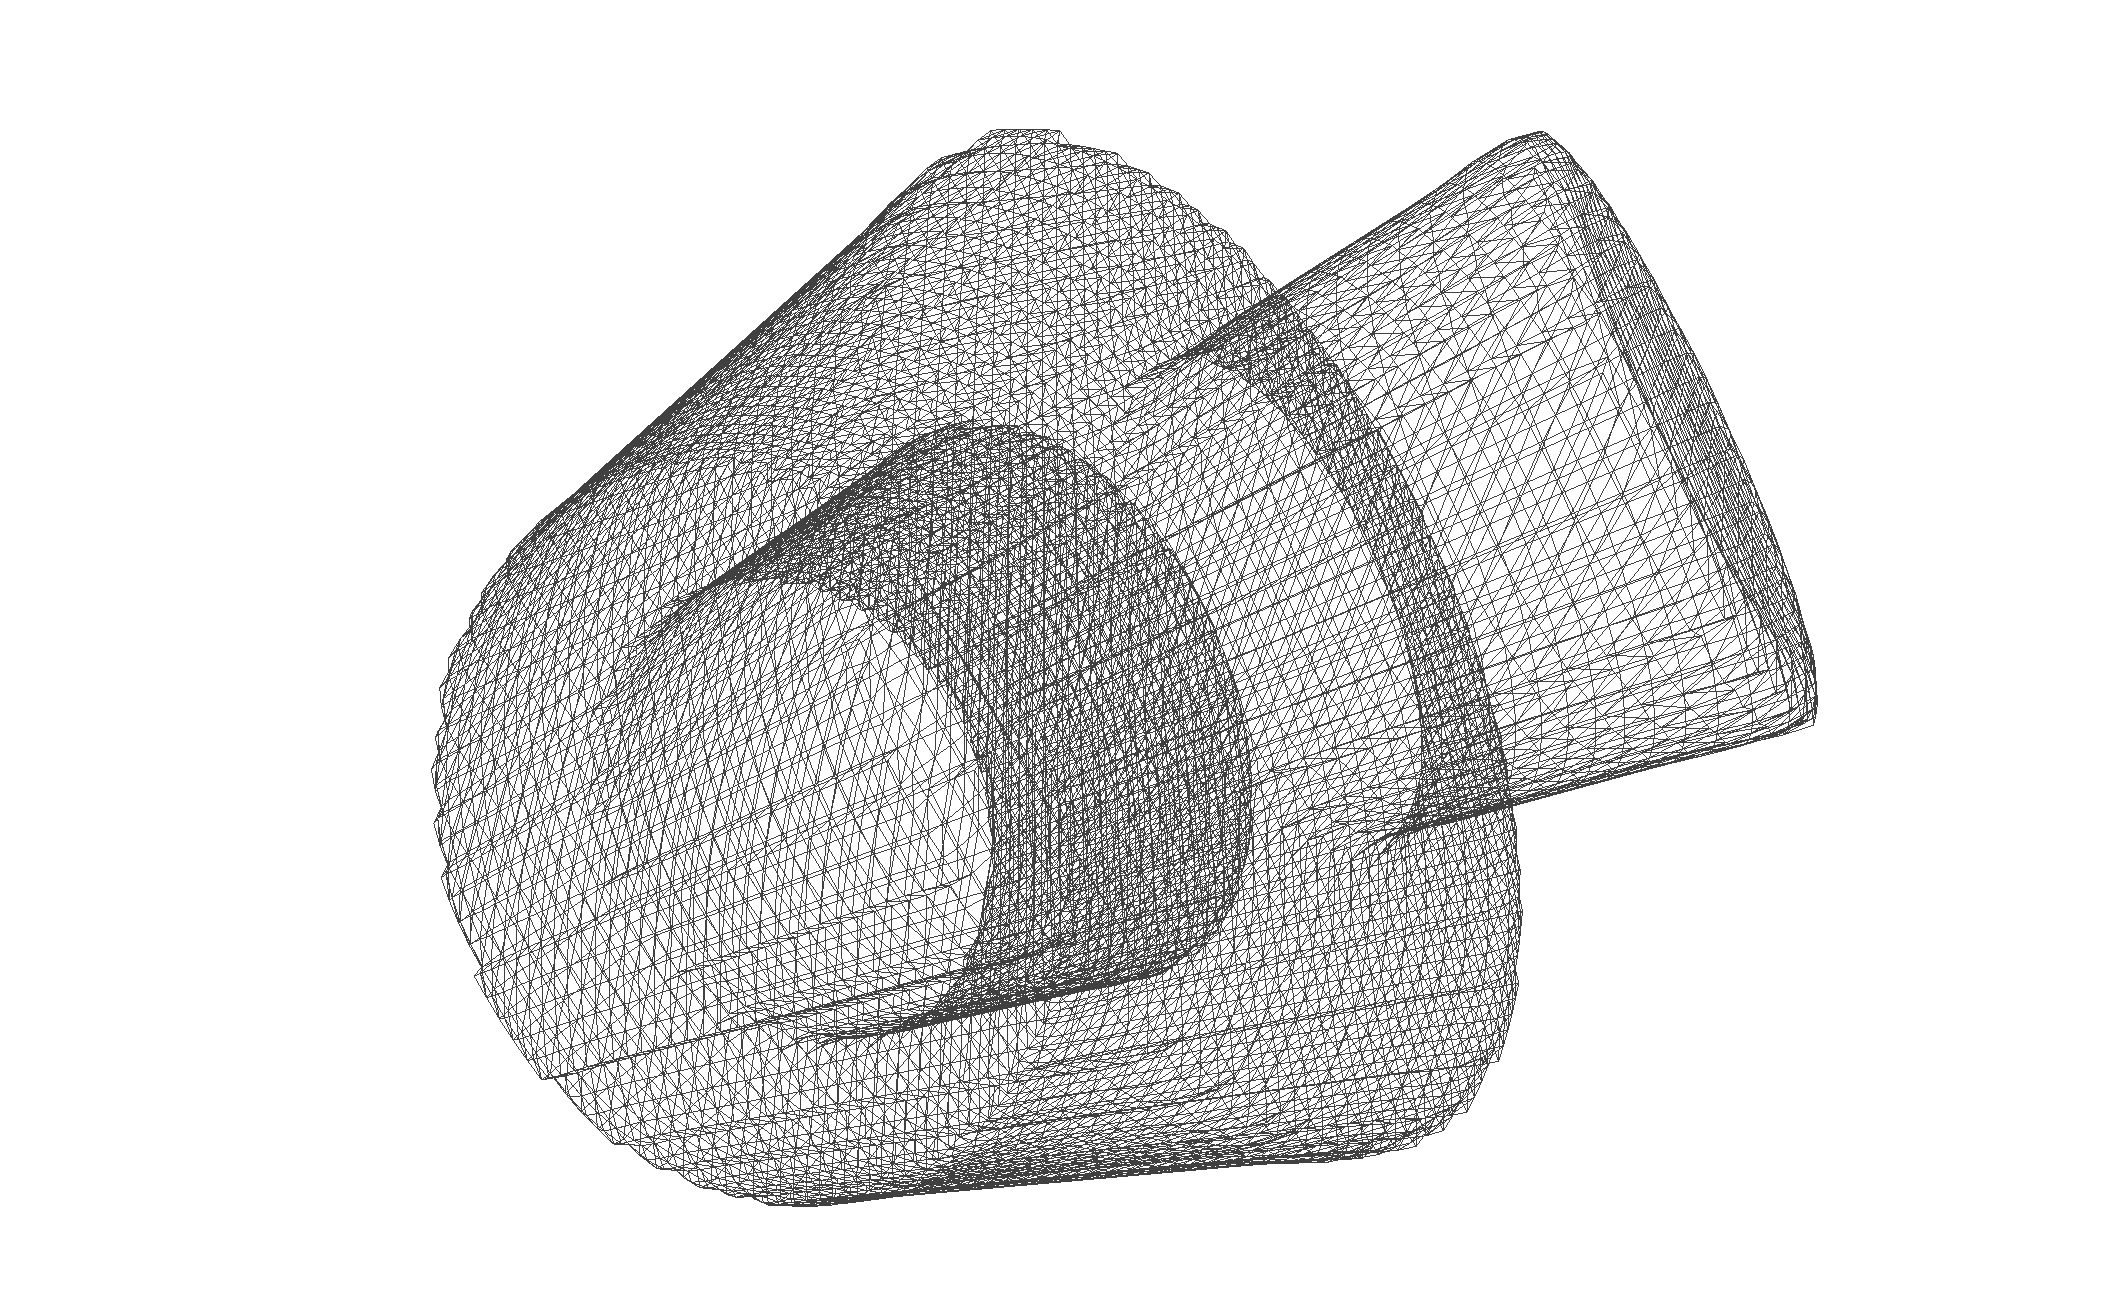
\includegraphics[width=0.25\linewidth]{7496_neural05.png}\\
            \shapeid{00008714} & 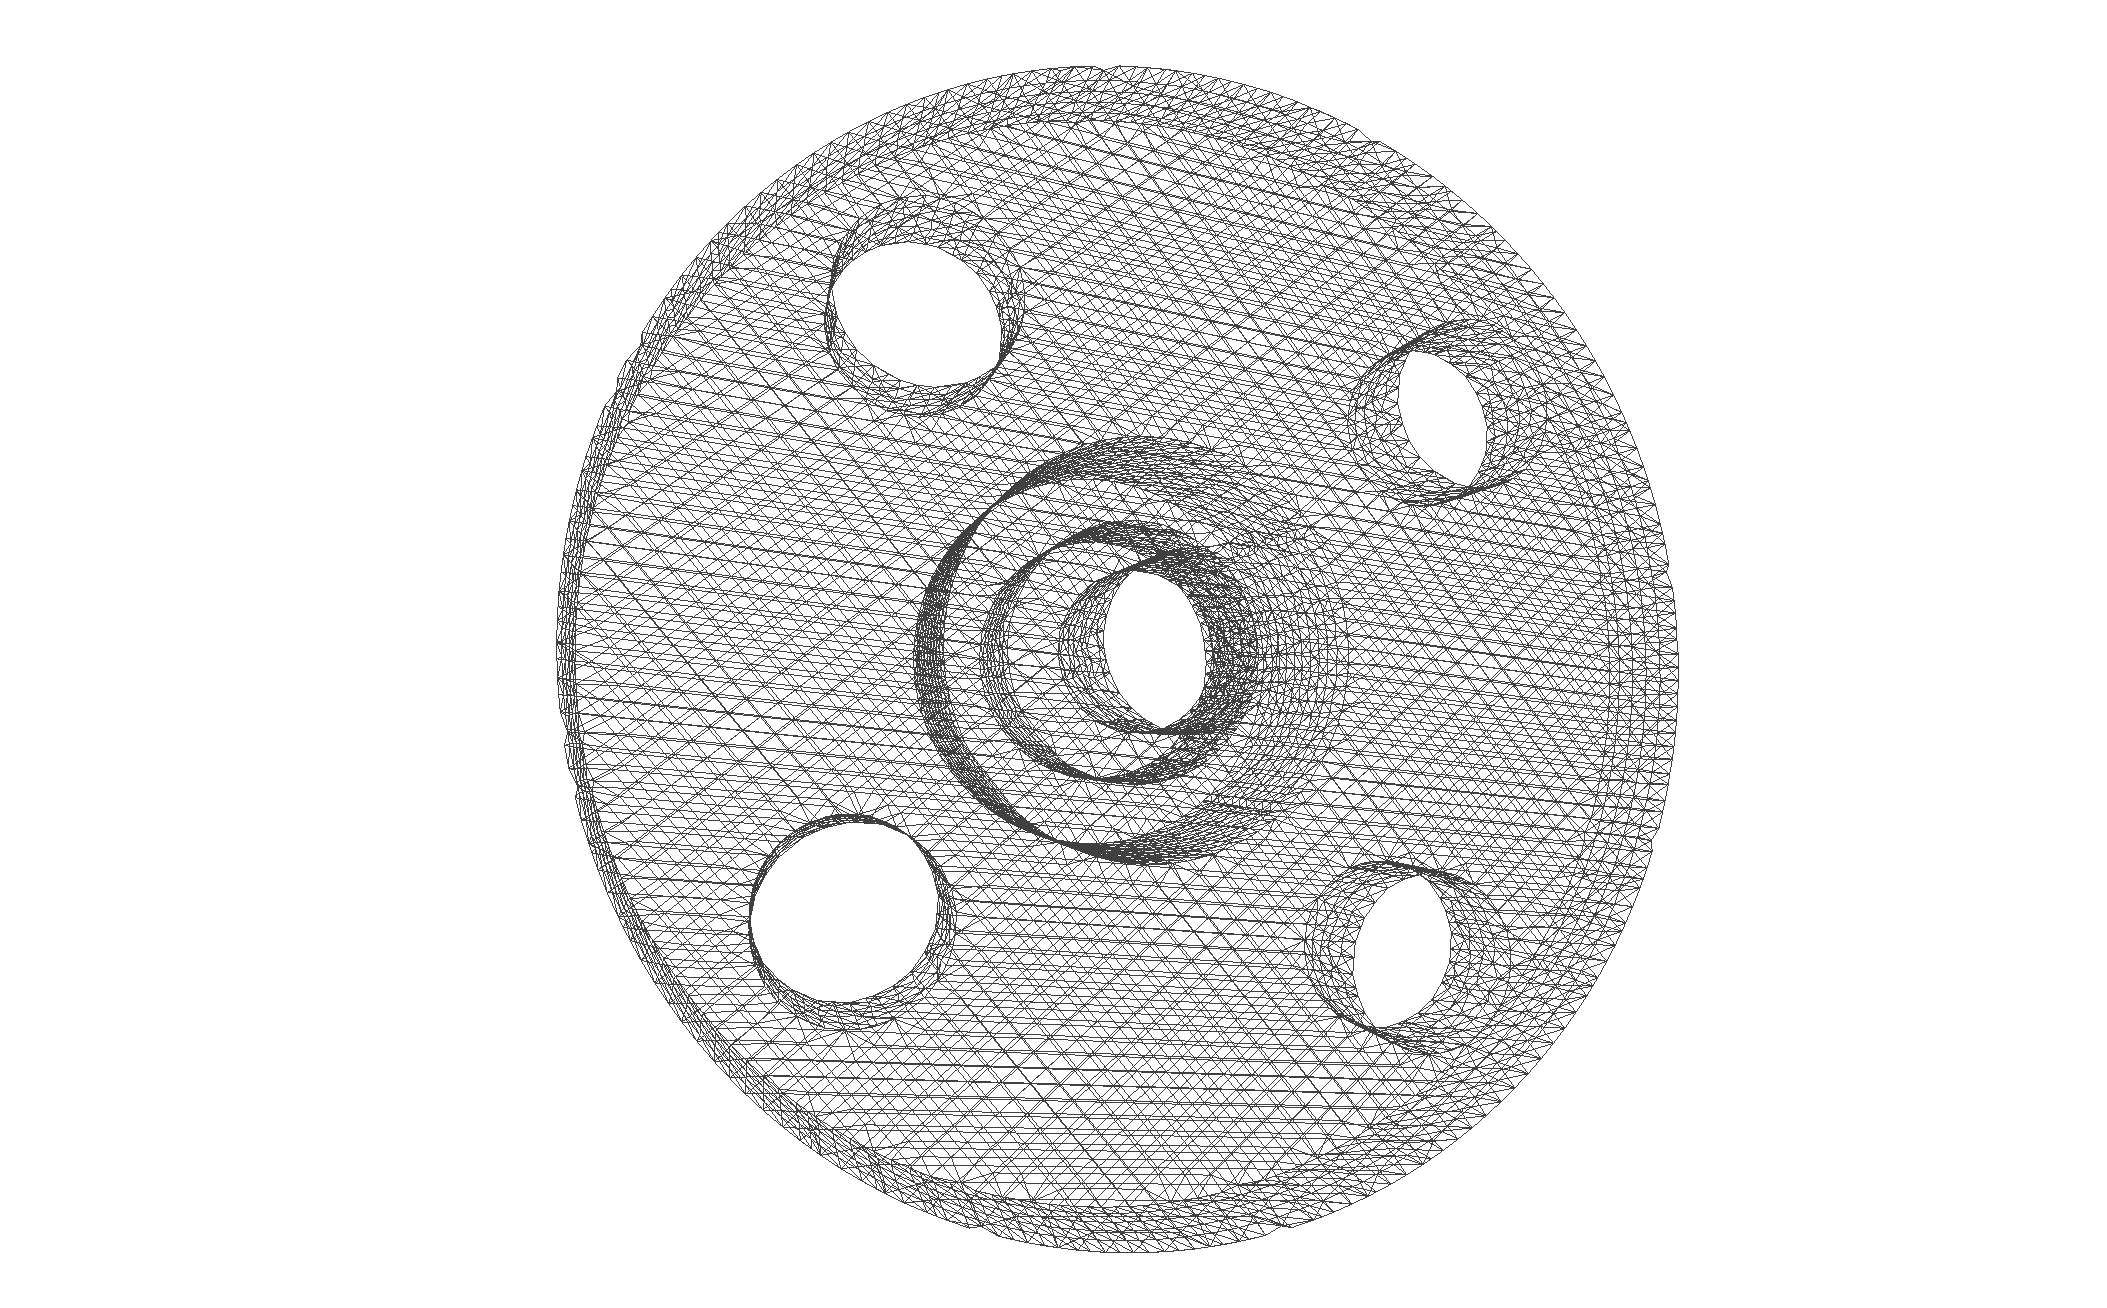
\includegraphics[width=0.25\linewidth]{8714_exact_p105.png} & 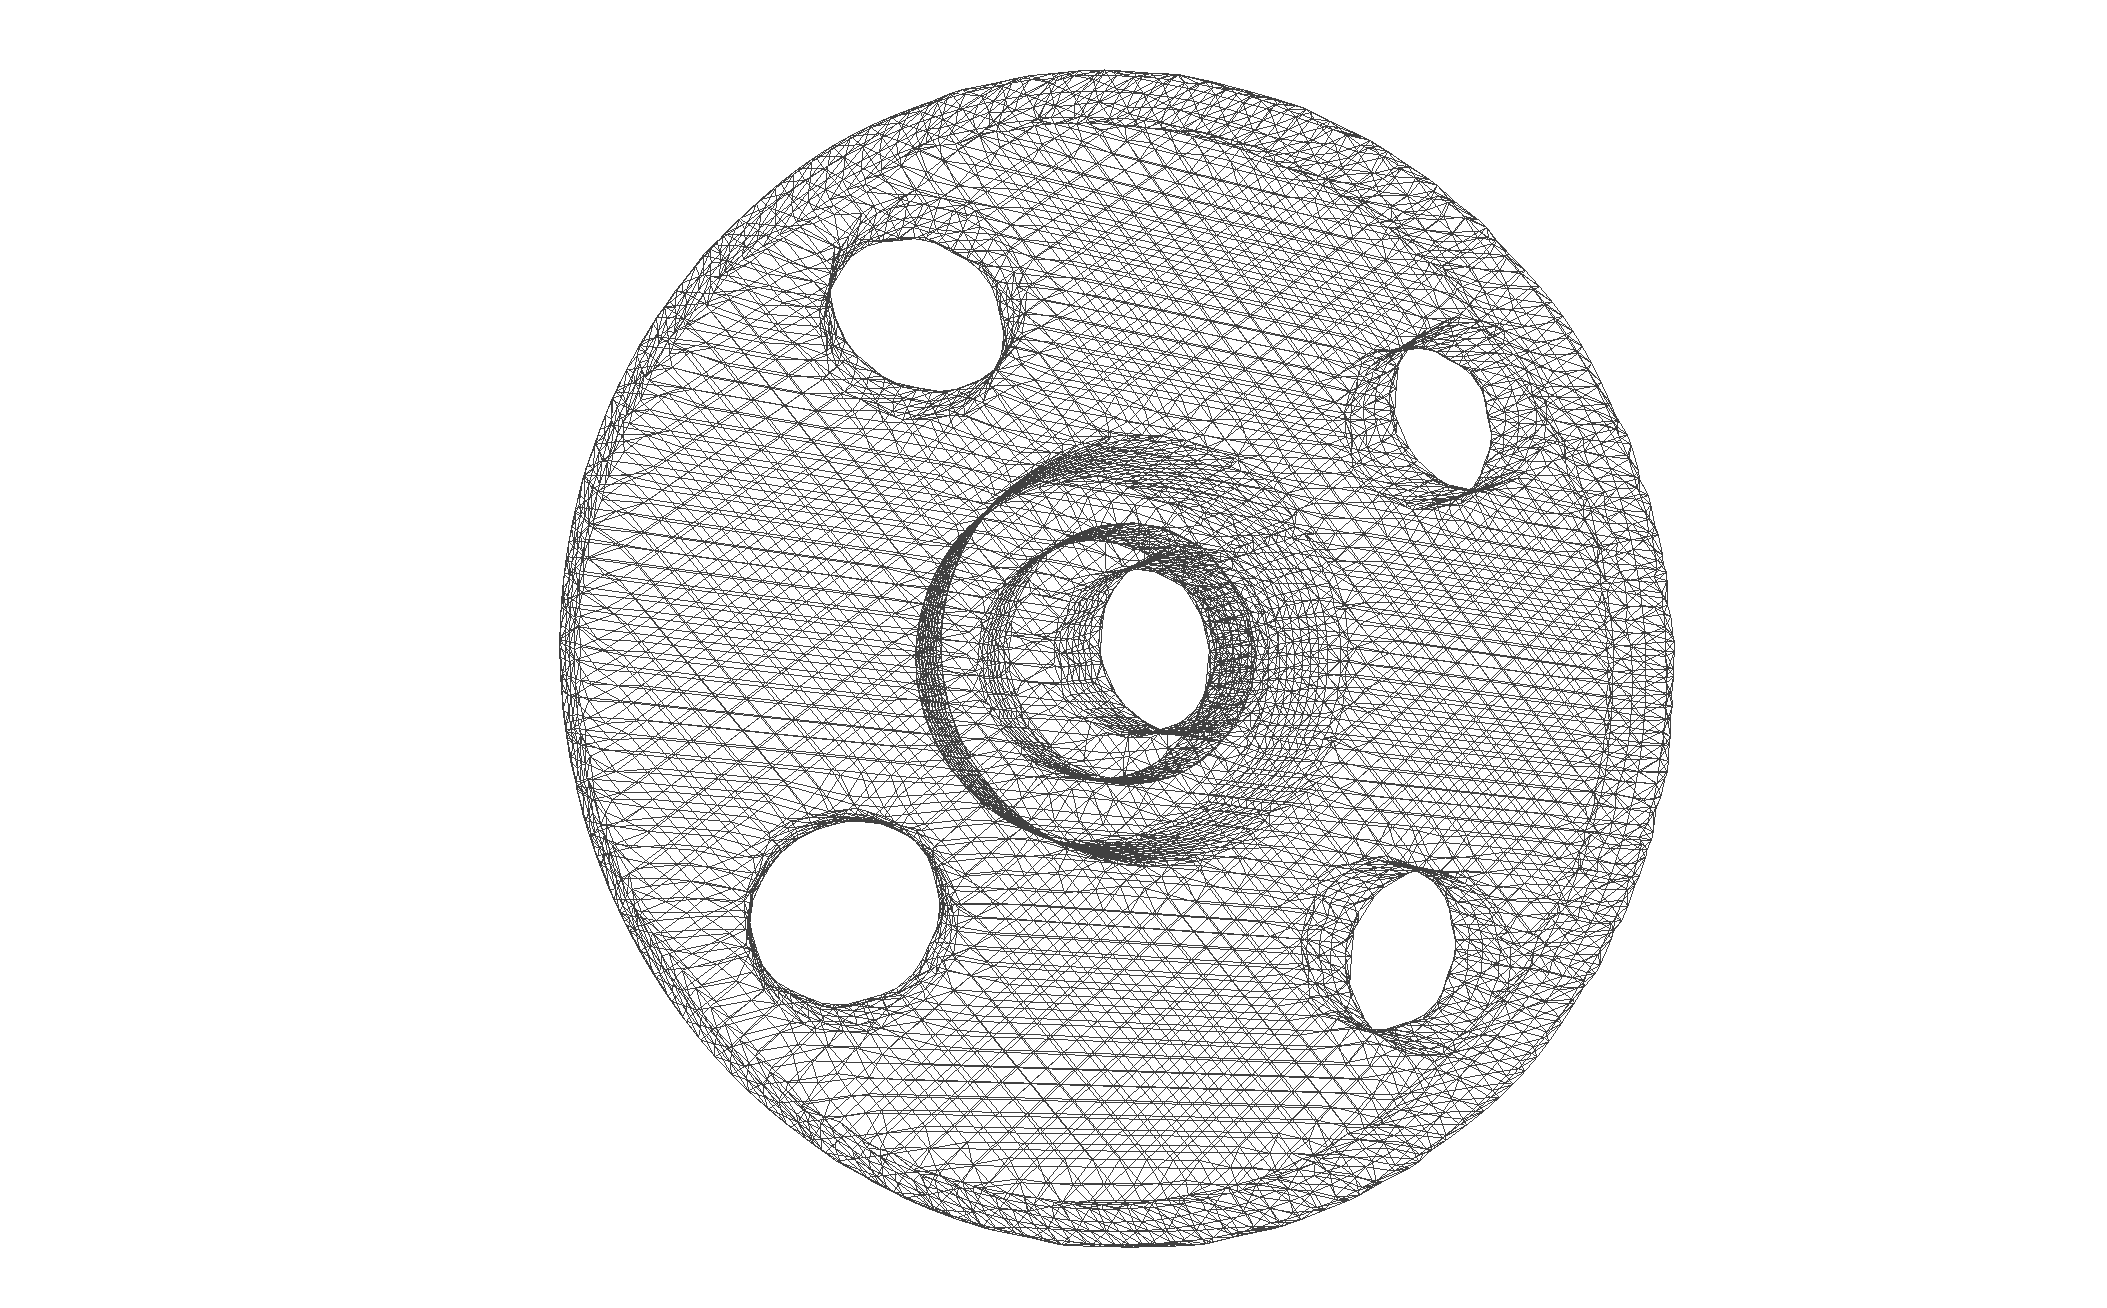
\includegraphics[width=0.25\linewidth]{8714_estimate_p106.png} & 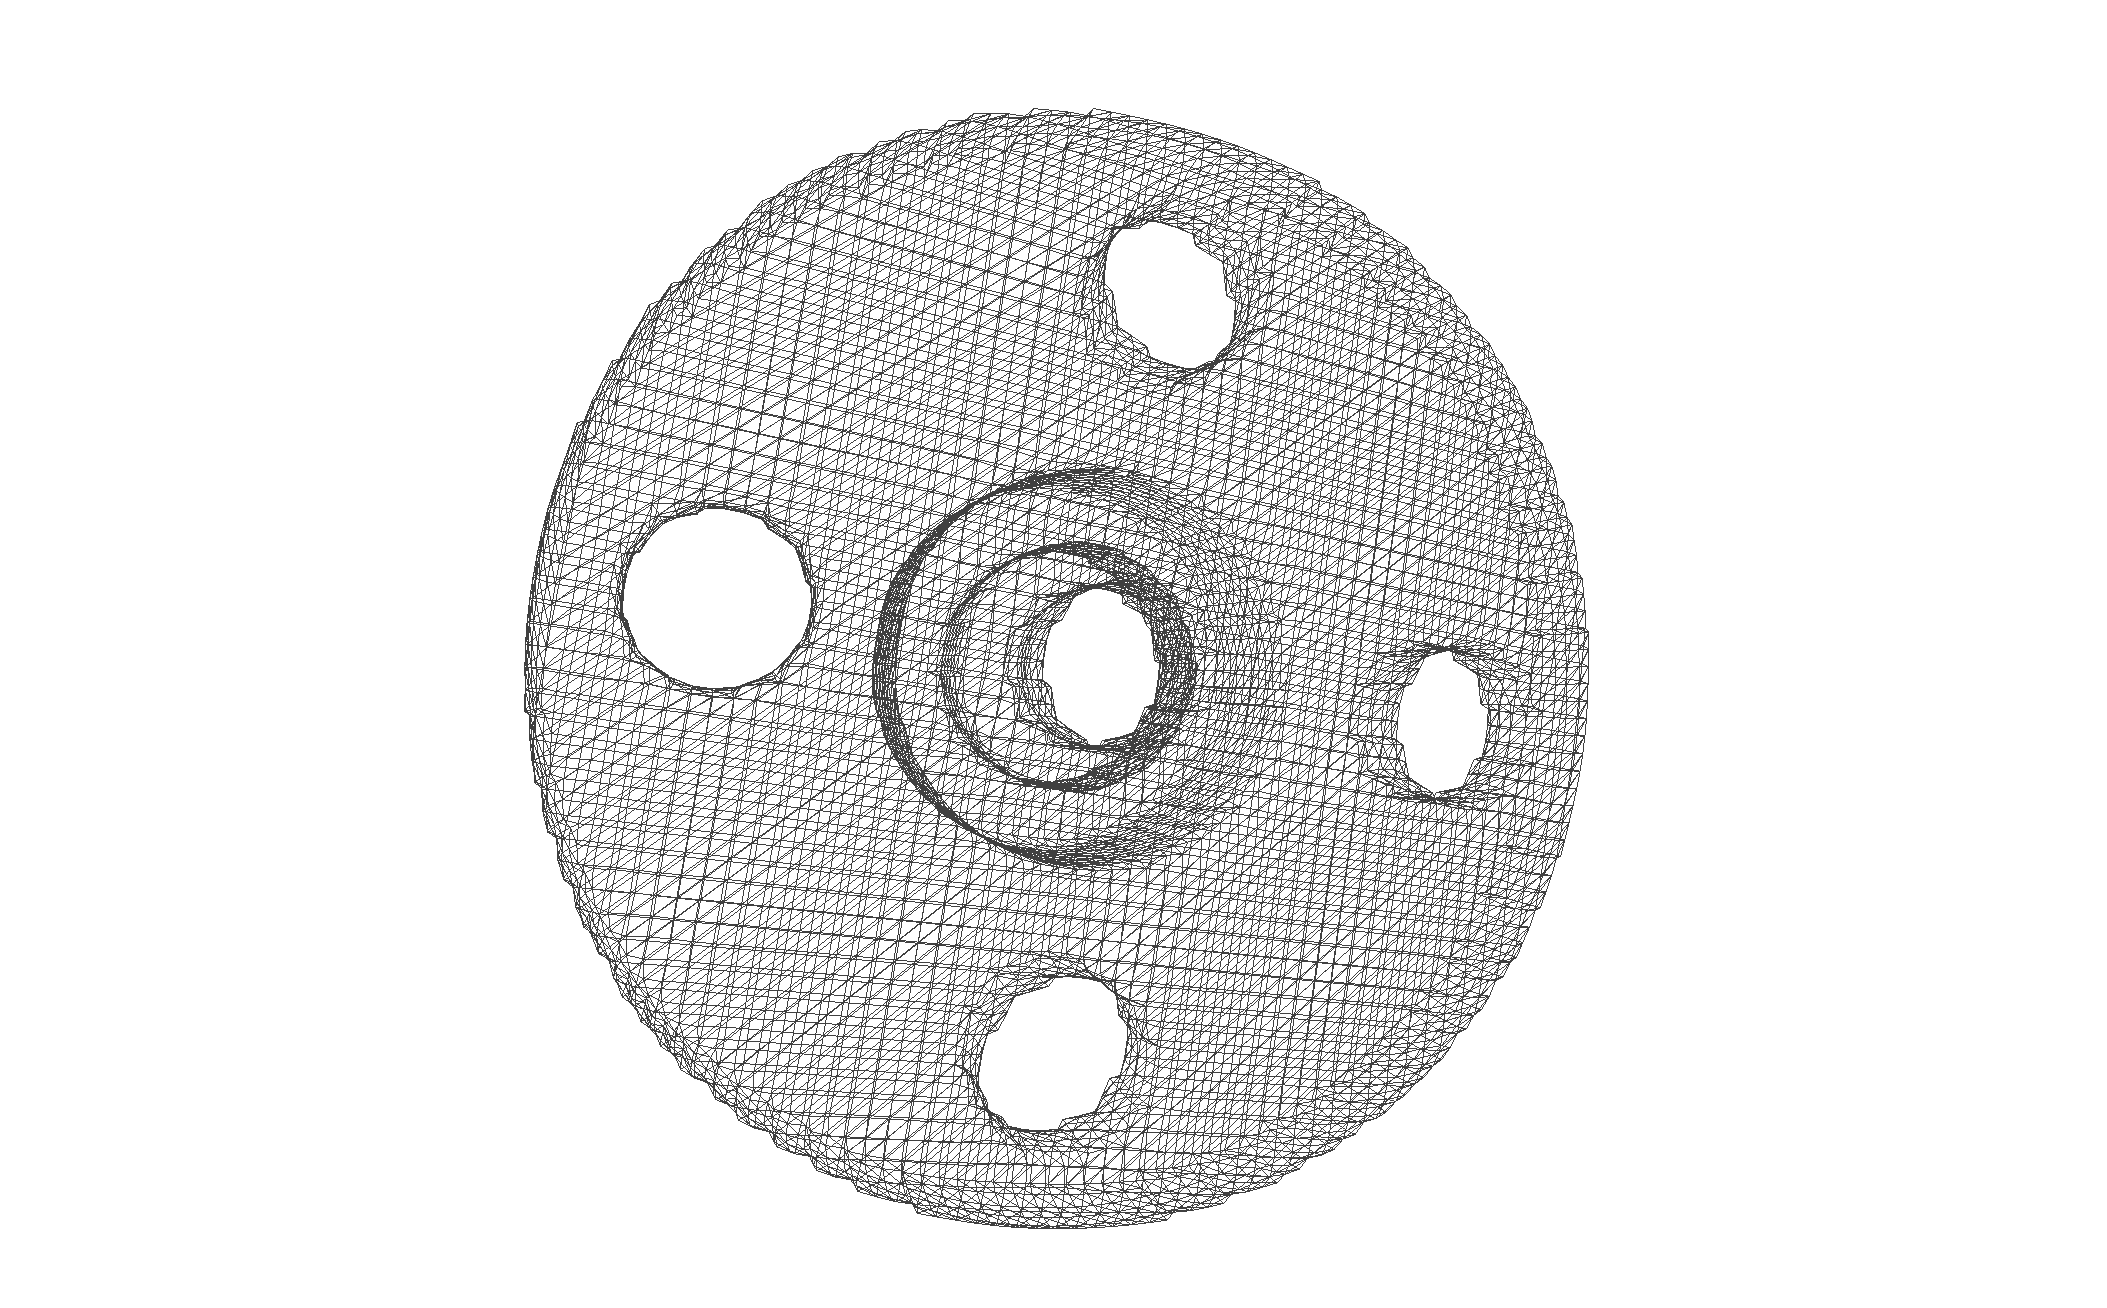
\includegraphics[width=0.25\linewidth]{8714_neural06.png}\\
            \shapeid{00009943} & 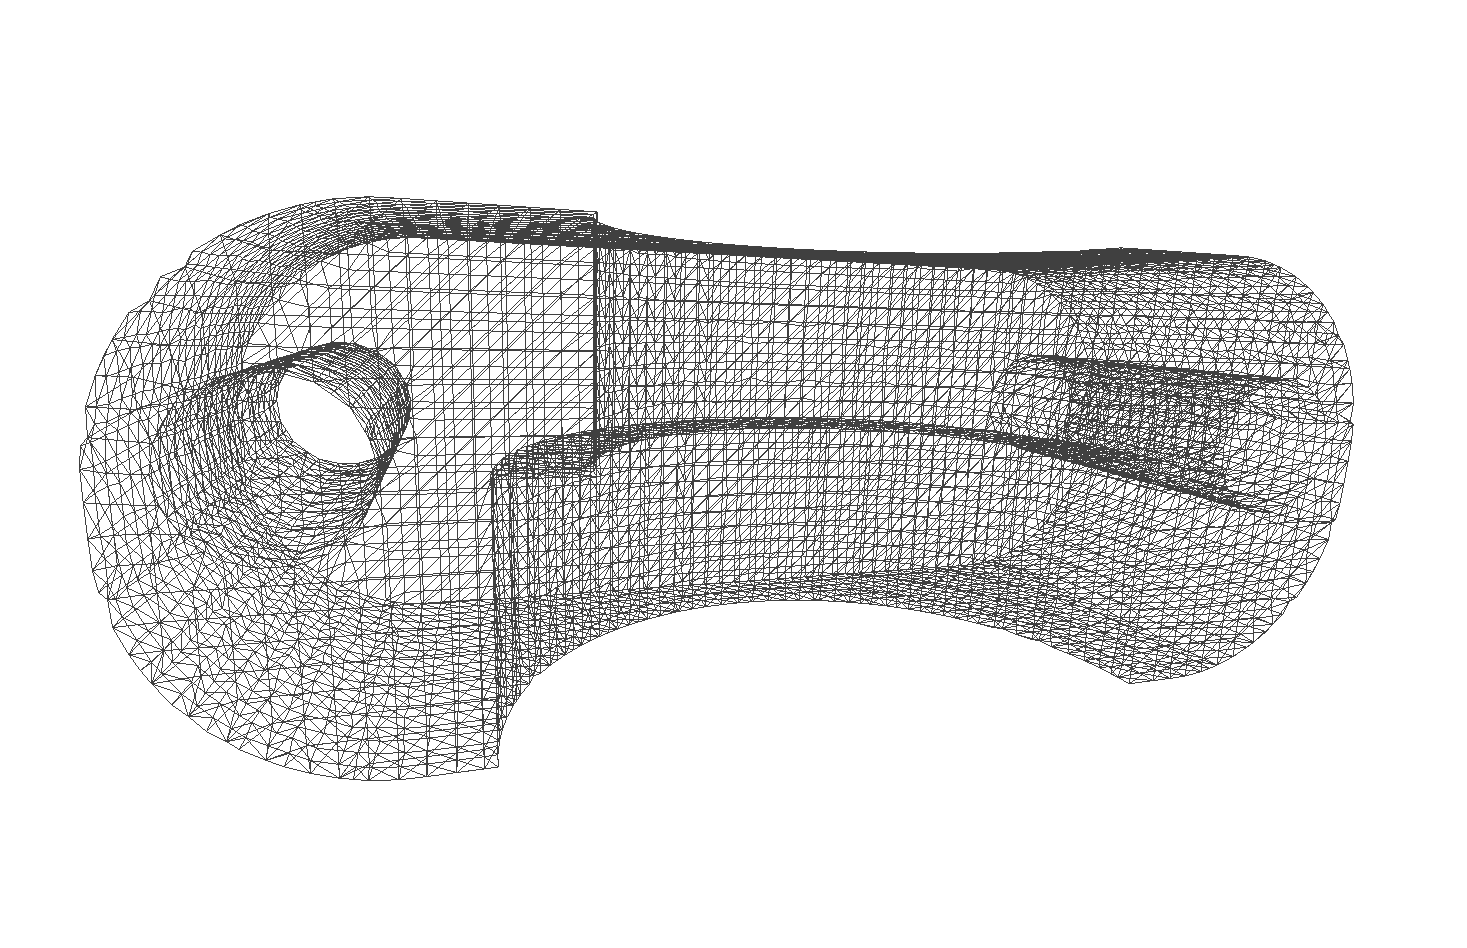
\includegraphics[width=0.25\linewidth]{9943_exact01.png } & 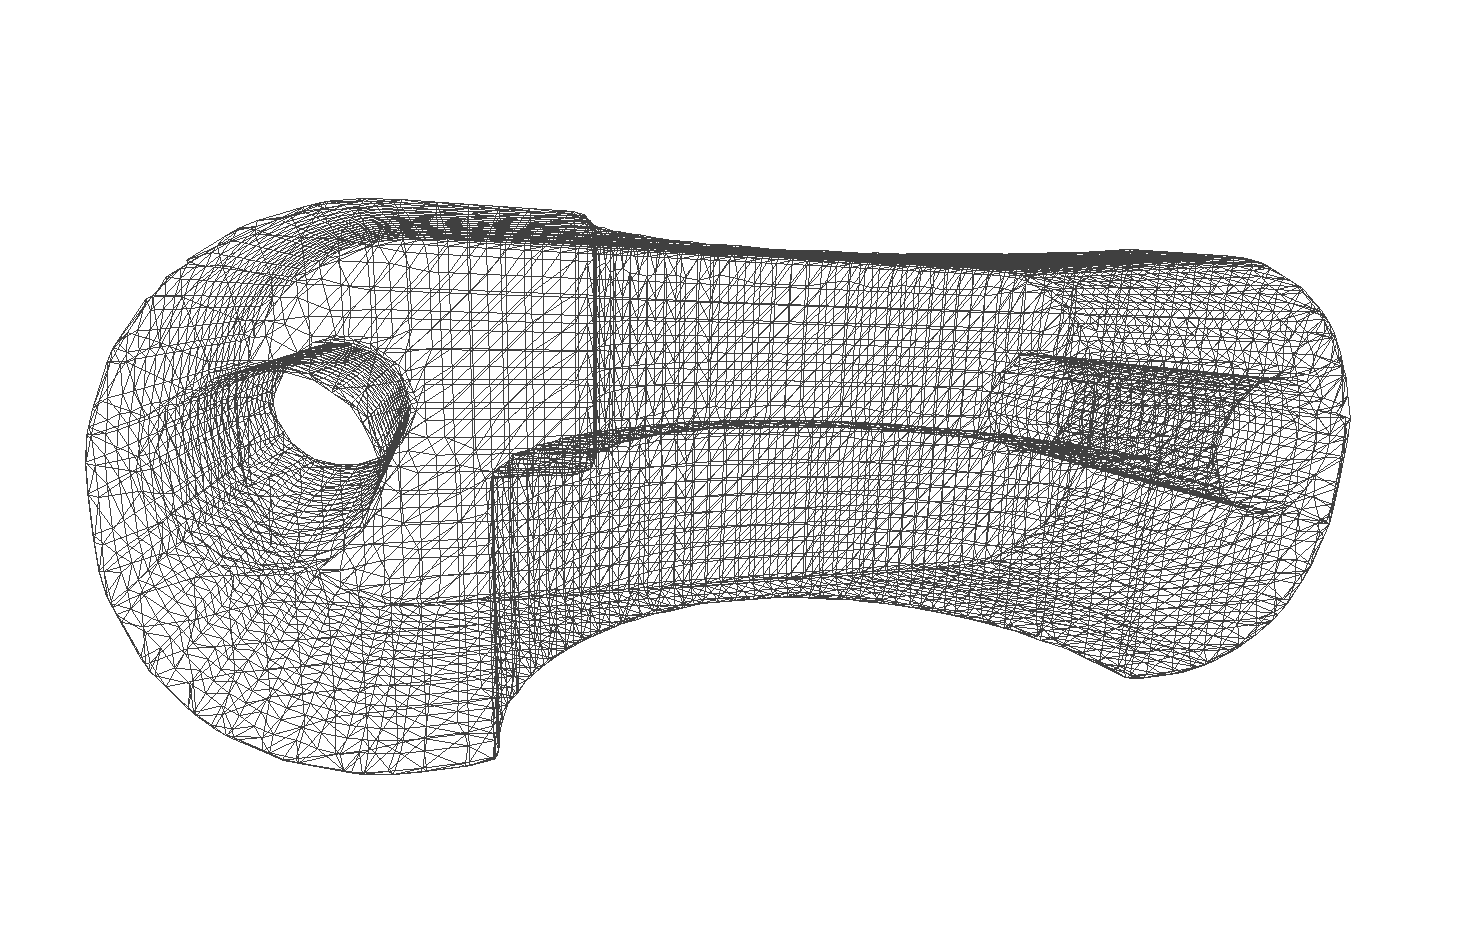
\includegraphics[width=0.25\linewidth]{9943_estimated00.png} & 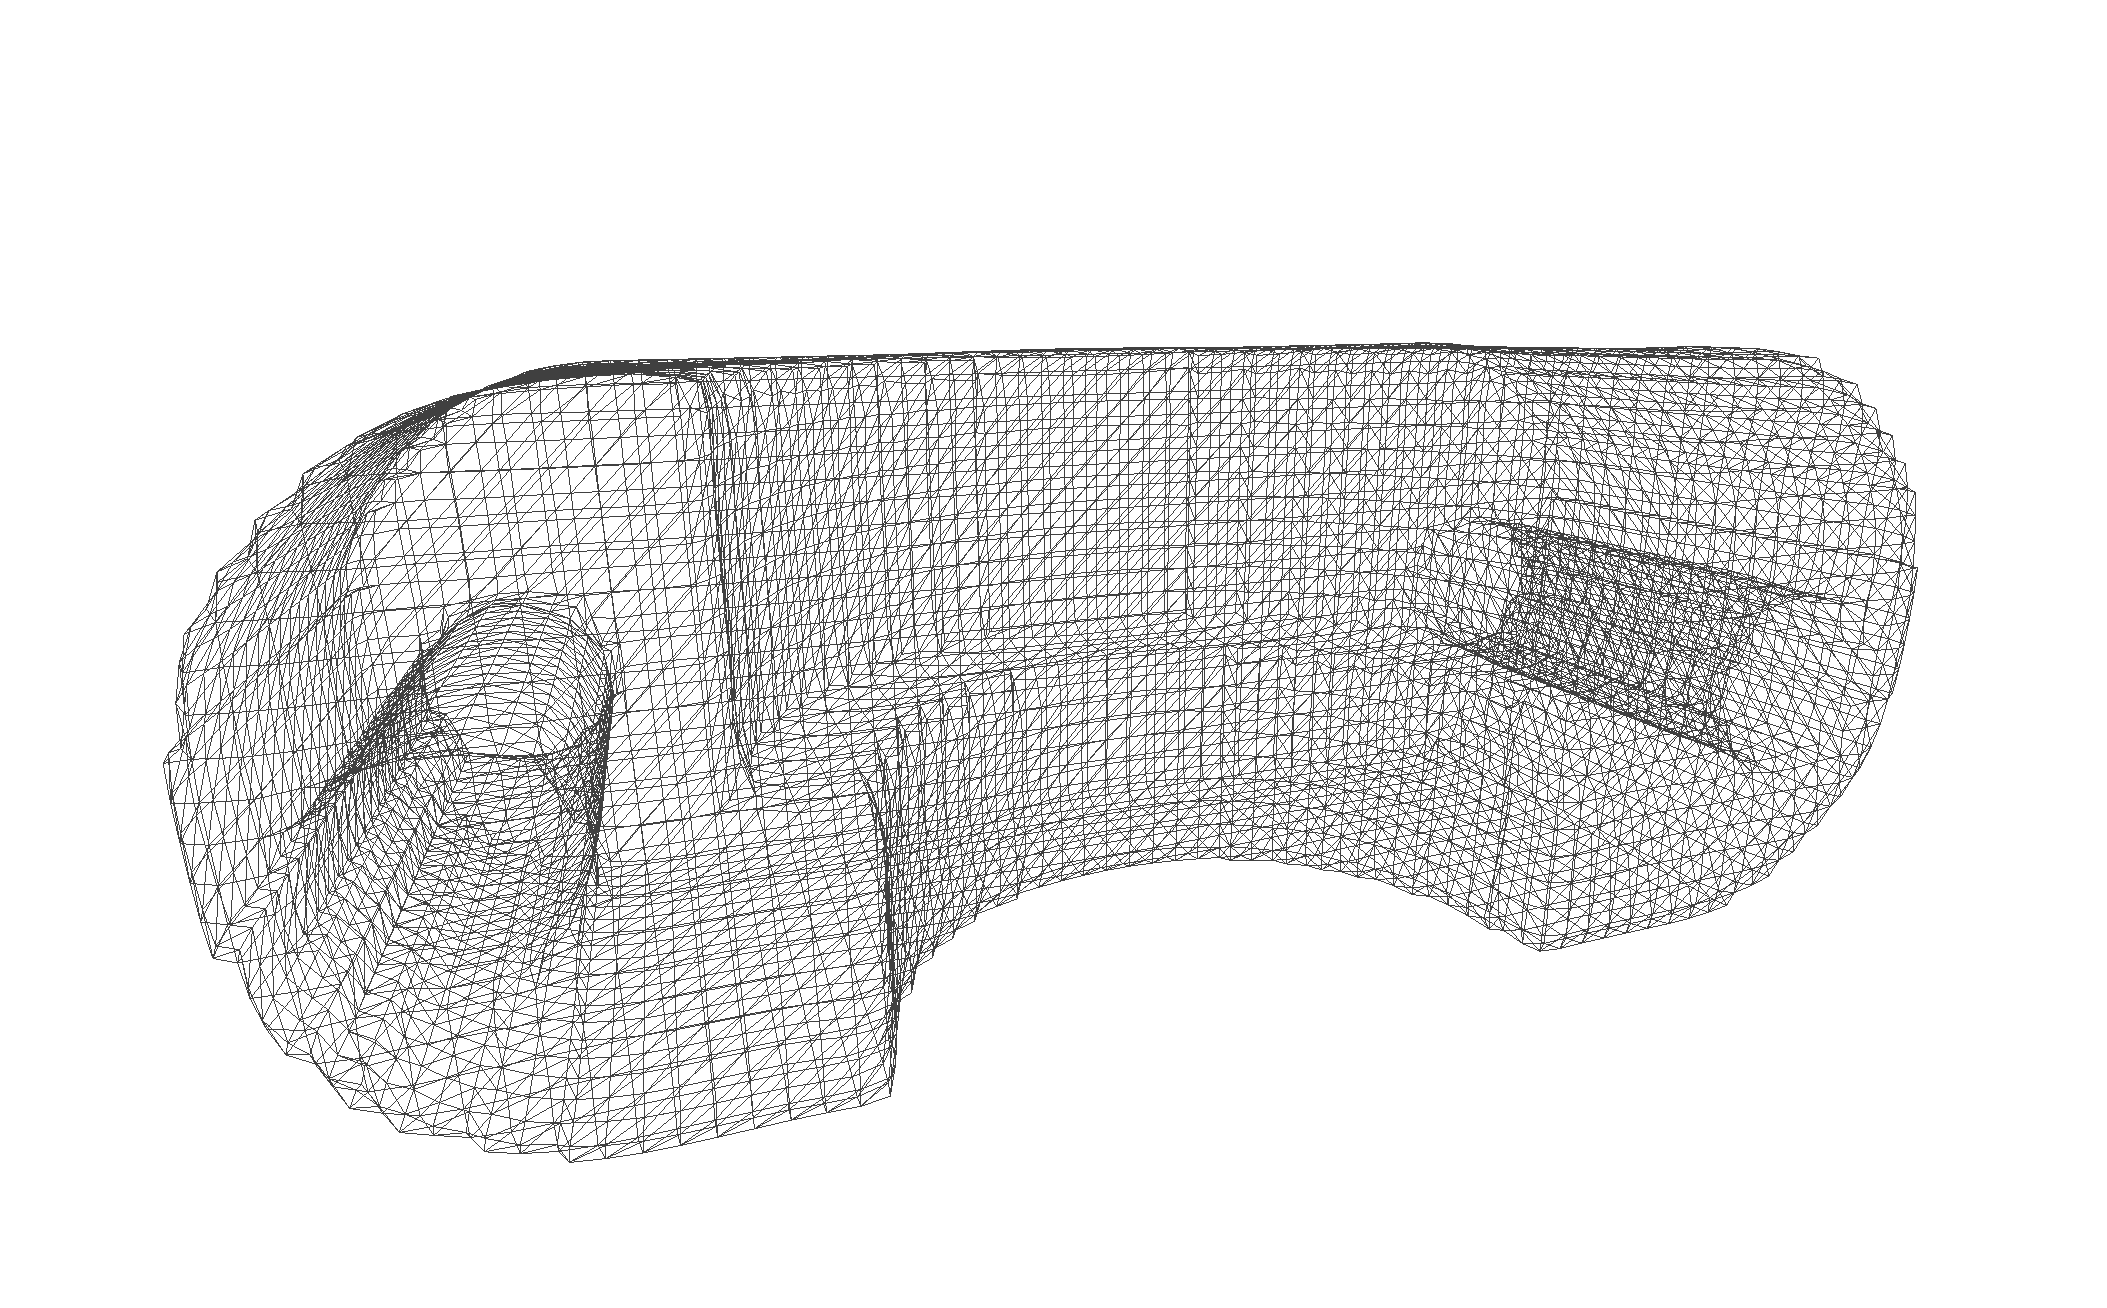
\includegraphics[width=0.25\linewidth]{9943_neural07.png}\\
      \end{tabular}
      \caption{Wireframe screenshots of the six evaluation shapes (rows) for each method (columns).}
      \label{fig:overview}
\end{figure}

\section*{Discussion}

When run on estimated hermite, the dual contouring mean
metric scores were 117.616\% worse for surface Chamfer Distance, and 163.946\% worse for edge CD compared to dual contouring with the exact hermite data. 
Visually though, they looked similar, where the main difference was the bumpier artifacts around curved edges, for example, the entrances and exits of the holes in 00004857.
This was present to a lesser degree in the exact hermite models, suggesting a native issue with dual contouring.

The differences were more pronounced with NDC compared to estimated hermite DC. Mean metric scores were
136.873\% for surface CD and 67.6297\% for edge CD. On flat and curved surfaces, there is was some stairstepping in the NDC result, and curved edges are again, not smooth.

In the interest of time I only ran neural dual contouring for 1000 steps. I would expect less jagged surfaces when running the default 10000 steps.



\clearpage

\end{document}
